% Options for packages loaded elsewhere
% Options for packages loaded elsewhere
\PassOptionsToPackage{unicode}{hyperref}
\PassOptionsToPackage{hyphens}{url}
\PassOptionsToPackage{dvipsnames,svgnames,x11names}{xcolor}
%
\documentclass[
  12pt,
]{article}
\usepackage{xcolor}
\usepackage[left=25mm,right=25mm,top=25mm,bottom=25mm]{geometry}
\usepackage{amsmath,amssymb}
\setcounter{secnumdepth}{-\maxdimen} % remove section numbering
\usepackage{iftex}
\ifPDFTeX
  \usepackage[T1]{fontenc}
  \usepackage[utf8]{inputenc}
  \usepackage{textcomp} % provide euro and other symbols
\else % if luatex or xetex
  \usepackage{unicode-math} % this also loads fontspec
  \defaultfontfeatures{Scale=MatchLowercase}
  \defaultfontfeatures[\rmfamily]{Ligatures=TeX,Scale=1}
\fi
\usepackage{lmodern}
\ifPDFTeX\else
  % xetex/luatex font selection
\fi
% Use upquote if available, for straight quotes in verbatim environments
\IfFileExists{upquote.sty}{\usepackage{upquote}}{}
\IfFileExists{microtype.sty}{% use microtype if available
  \usepackage[]{microtype}
  \UseMicrotypeSet[protrusion]{basicmath} % disable protrusion for tt fonts
}{}
\makeatletter
\@ifundefined{KOMAClassName}{% if non-KOMA class
  \IfFileExists{parskip.sty}{%
    \usepackage{parskip}
  }{% else
    \setlength{\parindent}{0pt}
    \setlength{\parskip}{6pt plus 2pt minus 1pt}}
}{% if KOMA class
  \KOMAoptions{parskip=half}}
\makeatother
% Make \paragraph and \subparagraph free-standing
\makeatletter
\ifx\paragraph\undefined\else
  \let\oldparagraph\paragraph
  \renewcommand{\paragraph}{
    \@ifstar
      \xxxParagraphStar
      \xxxParagraphNoStar
  }
  \newcommand{\xxxParagraphStar}[1]{\oldparagraph*{#1}\mbox{}}
  \newcommand{\xxxParagraphNoStar}[1]{\oldparagraph{#1}\mbox{}}
\fi
\ifx\subparagraph\undefined\else
  \let\oldsubparagraph\subparagraph
  \renewcommand{\subparagraph}{
    \@ifstar
      \xxxSubParagraphStar
      \xxxSubParagraphNoStar
  }
  \newcommand{\xxxSubParagraphStar}[1]{\oldsubparagraph*{#1}\mbox{}}
  \newcommand{\xxxSubParagraphNoStar}[1]{\oldsubparagraph{#1}\mbox{}}
\fi
\makeatother


\usepackage{longtable,booktabs,array}
\usepackage{calc} % for calculating minipage widths
% Correct order of tables after \paragraph or \subparagraph
\usepackage{etoolbox}
\makeatletter
\patchcmd\longtable{\par}{\if@noskipsec\mbox{}\fi\par}{}{}
\makeatother
% Allow footnotes in longtable head/foot
\IfFileExists{footnotehyper.sty}{\usepackage{footnotehyper}}{\usepackage{footnote}}
\makesavenoteenv{longtable}
\usepackage{graphicx}
\makeatletter
\newsavebox\pandoc@box
\newcommand*\pandocbounded[1]{% scales image to fit in text height/width
  \sbox\pandoc@box{#1}%
  \Gscale@div\@tempa{\textheight}{\dimexpr\ht\pandoc@box+\dp\pandoc@box\relax}%
  \Gscale@div\@tempb{\linewidth}{\wd\pandoc@box}%
  \ifdim\@tempb\p@<\@tempa\p@\let\@tempa\@tempb\fi% select the smaller of both
  \ifdim\@tempa\p@<\p@\scalebox{\@tempa}{\usebox\pandoc@box}%
  \else\usebox{\pandoc@box}%
  \fi%
}
% Set default figure placement to htbp
\def\fps@figure{htbp}
\makeatother


% definitions for citeproc citations
\NewDocumentCommand\citeproctext{}{}
\NewDocumentCommand\citeproc{mm}{%
  \begingroup\def\citeproctext{#2}\cite{#1}\endgroup}
\makeatletter
 % allow citations to break across lines
 \let\@cite@ofmt\@firstofone
 % avoid brackets around text for \cite:
 \def\@biblabel#1{}
 \def\@cite#1#2{{#1\if@tempswa , #2\fi}}
\makeatother
\newlength{\cslhangindent}
\setlength{\cslhangindent}{1.5em}
\newlength{\csllabelwidth}
\setlength{\csllabelwidth}{3em}
\newenvironment{CSLReferences}[2] % #1 hanging-indent, #2 entry-spacing
 {\begin{list}{}{%
  \setlength{\itemindent}{0pt}
  \setlength{\leftmargin}{0pt}
  \setlength{\parsep}{0pt}
  % turn on hanging indent if param 1 is 1
  \ifodd #1
   \setlength{\leftmargin}{\cslhangindent}
   \setlength{\itemindent}{-1\cslhangindent}
  \fi
  % set entry spacing
  \setlength{\itemsep}{#2\baselineskip}}}
 {\end{list}}
\usepackage{calc}
\newcommand{\CSLBlock}[1]{\hfill\break\parbox[t]{\linewidth}{\strut\ignorespaces#1\strut}}
\newcommand{\CSLLeftMargin}[1]{\parbox[t]{\csllabelwidth}{\strut#1\strut}}
\newcommand{\CSLRightInline}[1]{\parbox[t]{\linewidth - \csllabelwidth}{\strut#1\strut}}
\newcommand{\CSLIndent}[1]{\hspace{\cslhangindent}#1}



\setlength{\emergencystretch}{3em} % prevent overfull lines

\providecommand{\tightlist}{%
  \setlength{\itemsep}{0pt}\setlength{\parskip}{0pt}}



 


\usepackage{indentfirst}
\setlength{\parindent}{15pt}
\setlength{\parskip}{10pt}
\usepackage[font=small]{caption}  % Options: small, footnotesize, scriptsize, etc.
\usepackage[noblocks]{authblk}
\renewcommand*{\Authsep}{, }
\renewcommand*{\Authand}{, }
\renewcommand*{\Authands}{, }
\renewcommand\Affilfont{\small}
\makeatletter
\@ifpackageloaded{caption}{}{\usepackage{caption}}
\AtBeginDocument{%
\ifdefined\contentsname
  \renewcommand*\contentsname{Table of contents}
\else
  \newcommand\contentsname{Table of contents}
\fi
\ifdefined\listfigurename
  \renewcommand*\listfigurename{List of Figures}
\else
  \newcommand\listfigurename{List of Figures}
\fi
\ifdefined\listtablename
  \renewcommand*\listtablename{List of Tables}
\else
  \newcommand\listtablename{List of Tables}
\fi
\ifdefined\figurename
  \renewcommand*\figurename{Figure}
\else
  \newcommand\figurename{Figure}
\fi
\ifdefined\tablename
  \renewcommand*\tablename{Table}
\else
  \newcommand\tablename{Table}
\fi
}
\@ifpackageloaded{float}{}{\usepackage{float}}
\floatstyle{ruled}
\@ifundefined{c@chapter}{\newfloat{codelisting}{h}{lop}}{\newfloat{codelisting}{h}{lop}[chapter]}
\floatname{codelisting}{Listing}
\newcommand*\listoflistings{\listof{codelisting}{List of Listings}}
\makeatother
\makeatletter
\makeatother
\makeatletter
\@ifpackageloaded{caption}{}{\usepackage{caption}}
\@ifpackageloaded{subcaption}{}{\usepackage{subcaption}}
\makeatother
\usepackage{bookmark}
\IfFileExists{xurl.sty}{\usepackage{xurl}}{} % add URL line breaks if available
\urlstyle{same}
\hypersetup{
  pdftitle={Neural responses to binocular in-phase and anti-phase stimuli},
  pdfauthor={Bruno Richard; Daniel H. Baker},
  colorlinks=true,
  linkcolor={blue},
  filecolor={Maroon},
  citecolor={Blue},
  urlcolor={Blue},
  pdfcreator={LaTeX via pandoc}}


\title{Neural responses to binocular in-phase and anti-phase stimuli}

  \author[1]{Bruno Richard}
  \author[2]{Daniel H. Baker}

      \affil[1]{Department of Math and Computer Sciences, Rutgers
University, Newark, New Jersey, USA}
      \affil[2]{Department of Psychology, University of York, York, UK}
  
\date{}
\begin{document}
\maketitle
\begin{abstract}
VSS Abstract - Binocular vision fuses similar stimuli into a single
percept, yet incompatible stimuli result in other experiences such as
rivalry, lustre, and diplopia. We measured neural responses to binocular
stimuli with different phase relationships, intending to understand them
using contemporary binocular models. Steady-State Visually Evoked
Potentials (SSVEPs) were recorded from 15 observers in response to
monocular and binocular stimulation at 3Hz, using either on-off or
counterphase flicker. Across the eyes, binocular stimuli could be (i) in
spatial and temporal phase, (ii) in temporal phase but spatial
antiphase, (iii) in spatial phase but temporal antiphase, or (iv) in
spatial and temporal antiphase (for counterphase flicker this is
identical to condition (i)). Responses to monocular on-off flicker
showed peaks at the fundamental frequency (3Hz) and its harmonics
(integer multiples of 3Hz). In contrast, counterphase flicker produced
responses only at twice the flicker frequency (6Hz) and its harmonics.
Binocular in-phase stimulation resulted in a similar pattern of
responses, consistent with `ocularity invariance' -- the observation
that binocular and monocular stimuli appear equal at high contrasts.
Changing the phase relationship modulated the harmonics pattern in
complex ways. On-off flicker in temporal antiphase reduced the
fundamental response, but there was no such effect for counterphase
flicker. We modelled the data using a progression of binocular
combination algorithms that increased in complexity from a simple linear
sum to a two-stage binocular gain control model with parallel monocular
and binocular phase-selective channels (the Lustre model). The most
complex model (lustre) outperformed all other models in capturing the
variance of our SSVEP data, although simpler phase-insensitive models
performed similarly well in most experimental conditions. Simpler models
struggled to capture the response magnitude to counterphase stimuli. Our
findings suggest that explaining neural responses to binocular stimuli
with different phase relationships requires parallel monocular and
phase-selective channels.
\end{abstract}


\section{Introduction}\label{introduction}

The human visual system integrates input from both eyes to form a
unified binocular representation of the world. Combining monocular
inputs enhances sensitivity to the presented stimuli, particularly when
the contrast is low or near detection threshold (Baker et al., 2018;
Campbell and Green, 1965; Meese et al., 2006). Contrast sensitivity can
improve by a factor of \(\sqrt{2}\) or more when stimuli are presented
binocularly versus monocularly (Baker et al., 2018; Blake and Wilson,
2011; Campbell and Green, 1965; Richard et al., 2018). Notably, the
visual system also attempts to combine inputs even when the stimuli
presented to each eye are markedly different (i.e., incompatible). In
such cases, observers may perceive binocular rivalry (Blake, 1989;
Wilson, 2003), diplopia, or visual lustre (Georgeson et al., 2016).
Despite differences in perceptual outcomes, computationally, the
underlying processes of binocular combination for compatible and
incompatible inputs appear similar (Baker et al., 2007a; Legge, 1984).
Human behavioural responses to compatible and incompatible stimuli can
be effectively explained by a single psychophysical model that involves
nonlinear transduction, followed by summation across monocular and
binocular phase-selective channels (Baker et al., 2007a; Baker and
Meese, 2007). Here we explore if the integrative processes defined over
multiple behavioural tasks are also reflected at the neural level.

It has long been known that stimuli presented binocularly are summed
across the eyes. In contrast detection tasks, where stimulus contrast is
low, binocular presentation increases sensitivity by approximately
\(\sqrt{2}\) (Campbell and Green, 1965). This implies that observers
require roughly 1.4 times more contrast to detect a monocular stimulus
than a binocular one. The binocular improvement in sensitivity is
consistent with a non-linearity operating before the signals from the
two eyes (\(C_L\) and \(C_R\)) are combined (Legge, 1984):
\begin{equation}\phantomsection\label{eq-IntroMath1}{
R_B = C_L^m + C_R^m.
}\end{equation} Here, the exponent \(m\) determines the degree of
summation. When \(m = 1\), summation is linear, yielding a doubling of
sensitivity. When \(m = 2\), summation is reduced to \(\sqrt{2}\).
Several studies have reported summation ratios over \(\sqrt{2}\) with
some approaching 1.8 (Meese et al., 2006; Simmons, 2005; Simmons and
Kingdom, 1998). A recent meta-analysis of 65 studies (N = 716) found an
average binocular summation ratio of 1.5 (Baker et al., 2018). This work
highlighted the challenges in accurately describing the binocular
summation process (e.g., \(m\)) as individual variability and
methodological differences can greatly impact binocular summation.

The contrast of stimuli, for example, is crucial in measuring binocular
summation. Binocular summation can be very large when stimulus contrast
is low; however, the binocular advantage is seldom observed in tasks
that involve higher contrasts. In contrast discrimination tasks, where
observers judge the contrast difference between otherwise identical
stimuli, binocular presentation no longer confers a benefit in
sensitivity (Legge, 1984; Maehara and Goryo, 2005; Meese et al., 2006):
discrimination thresholds are identical whether stimuli are shown to one
eye or both. This does not mean binocular signals are not combined at
higher contrasts (Meese et al., 2006; Meese and Baker, 2011). Instead,
the advantage of summation is counteracted by normalization mechanisms
that maintain consistency across viewing conditions (referred to as
`ocularity invariance'). In contrast gain control models of early
vision, normalization can stem from interocular and self-suppressive
signals (Meese et al., 2006):
\begin{equation}\phantomsection\label{eq-intoMath2}{
R_B = \frac{C_L^m}{S+C_L+C_R} + \frac{C_R^m}{S+C_R+C_L}.
}\end{equation} When both eyes are stimulated, the suppressive terms on
the denominators offset the enhanced excitatory signals, nullifying the
binocular advantage.

\textbf{Differencing Mechanisms?}

A similar pattern of results is observed in neural measurements of
binocular summation. In fMRI recordings, neural responses are
significantly larger for binocular than monocular responses when
stimulus contrast is low (Moradi and Heeger, 2009). At higher contrasts,
observers no longer show the binocular advantage. These findings were
well-explained by a model including interocular suppression and
binocular contrast normalization, an identical mechanism to that used to
explain behavioural data. The equivalency in binocular summation between
psychophysics and neuroimaging findings means that both data types can
be used to constrain binocular summation models. We, for example, have
previously demonstrated that a popular model of binocular summation
could be easily adapted to capture Steady-State Visually Evoked
Potentials (SSVEPs) to monocular and binocular stimuli when one eye was
occluded by a neutral density filter (Richard et al., 2018). Placing a
neutral density filter in front of one eye darkens its input, reducing
the amplitude and altering the phase of SSVEPs to stimuli presented to
the filtered eye. Steady-State response amplitudes and phases to stimuli
presented through different neutral density filter strengths were well
described by a model that first used a biophysically plausible temporal
filter on the input stimuli, followed by self and interocular
suppression, and finally, binocular contrast normalization. This model
also captures psychophysically measured binocular summation in the same
group of observers. A comprehensive description of the processes
involved in binocular summation should be able to explain behavioural
and neuroimaging findings under various experimental conditions of
binocular summation.

Many studies have worked towards the development of a comprehensive
description of the process of binocular summation in human vision using
a variety of psychophysical and neuroimaging data (Baker et al., 2008,
2007b; Ding et al., 2013; Ding and Sperling, 2006; Legge, 1984; Lygo et
al., 2021; Maehara and Goryo, 2005; Richard et al., 2018). Developing
these models is not an insignificant challenge; they must account for
multiple components of early vision, including identifying relevant
signals, defining how these signals might interact, what non-linearities
are present, and most importantly, how they are combined. One such model
that has proven very informative and capable of describing binocular
summation under various experimental conditions is the two-stage
contrast gain control model developed by Meese et al. (2006). The model
captured detection and discrimination thresholds for monocular and
binocular stimuli in addition to dichoptic stimuli, whereby the stimuli
presented to both eyes are not identical, in a two-stage process. First,
the input is rectified by an excitatory non-linearity
(\(m \approx 1.3\)) and normalized by self and interocular suppression
(see Equation~\ref{eq-intoMath2}). The binocular (e.g., combined) input
undergoes a second contrast normalization before the decision stage,
\begin{equation}\phantomsection\label{eq-IntroMathSecondStage}{
R = \frac{R_B^p}{Z + R_B^q},
}\end{equation} where the excitatory exponent \(p\) allows for greater
increase in sensitivity than would be seen by the excitatory
non-linearity of the first stage (\(m\) in Equation~\ref{eq-intoMath2})
alone.

Subsequent iterations of the two-stage contrast gain control model added
channels for opposite contrast polarities (Baker and Meese, 2007), and
monocular channels parallel the binocular summing channel (Georgeson et
al., 2016). Polarity-specific channels were included to explain masking
effects when the stimuli presented to each eye had opposing phase
polarities (i.e., dichoptic presentation). The presentation of
sinusoidal gratings with opposite polarities to each eye does not cancel
them out: stimuli remain detectable and the two inputs sum, albeit
weakly (Bacon, 1976; Baker and Meese, 2007; Simmons, 2005). Parallel
monocular channels were added to account for adaptation after-effects
that suggest monocular signals may be preserved and available for
perception following binocular summation (Blake et al., 1981; Moulden,
1980). While the possibility of monocular channels had been considered
(Legge, 1984), many assumed that only the binocularly summed signal
contributed to perception. In a comprehensive study of binocular
contrast perception, Georgeson et al. (2016) developed a specific
experimental condition to assess the involvement of monocular channels.
They devised a discrimination task where the target interval presented a
contrast increment to one eye (e.g., 10\% pedestal + 2\%) and a contrast
decrement to the other (e.g., 10\% pedestal - 2\%). If the only
available signal is a binocularly summed one, the task would be nearly
impossible to complete; the target interval would be perceptually
identical to the pedestal-only interval. However, observers were able to
complete the task. The two-stage contrast gain control model with
parallel monocular channels was the only model able to capture observer
thresholds from all experimental conditions, including the binocular
increment and decrement condition.

The current architecture of the two-stage contrast gain control model
has been rigorously evaluated on psychophysical data, providing a solid
foundation for our understanding of binocular combination (Baker and
Meese, 2007; Georgeson et al., 2016; Meese et al., 2006). While previous
studies have utilized the two-stage contrast gain control model on
neuroimaging data (Lygo et al., 2021; Richard et al., 2018), they only
included experimental conditions where the phases of the sinusoidal
gratings presented to each eye were identical. To accurately assess the
current architecture of the two-stage contrast gain control model,
neuroimaging data for binocular presentation of stimuli in opposite
phase polarity are required. Here, we recorded SSVEPs to monocular and
binocular stimuli with different spatial and temporal phase
relationships to obtain the data needed to evaluate the two-stage
contrast gain control model. By progressively increasing the complexity
of the model, we demonstrate that many mechanisms of binocular
combination, such as monocular non-linearities, interocular
interactions, and parallel monocular channels, are required to explain
neural responses to our set of experimental conditions. Thus, the
two-stage contrast gain control model remains a powerful and flexible
descriptor of the architecture of binocular combination for data
collected across many experimental conditions and modalities.

\section{Methods}\label{methods}

\subsection{Participants}\label{participants}

Fifteen observers (including both authors: BR and DHB) with normal or
corrected to normal visual acuity and binocular vision participated in
our study. Written informed consent was obtained from all participants,
and experimental procedures were approved by the ethics committee of the
Department of Psychology at the University of York.

\subsection{Apparatus}\label{apparatus}

All stimuli were presented using a gamma-corrected ViewPixx 3D display
(VPixx Technologies, Canada) driven by a Mac Pro. Binocular separation
with minimal crosstalk was achieved by synchronizing the display's
refresh rate with the toggling of a pair of Nvidia stereo shutter
goggles using an infrared signal. The monitor refresh rate was set to
120 Hz; each eye updated at 60 Hz (every 16.67 msec). The display
resolution was set to 1920 X 1080 pixels. A single pixel subtended
0.027\(^o\) of visual angle (1.63 arc min) when viewed from 57 cm. The
mean luminance of the display viewed through the shutter goggles was 26
cd/m\(^2\).

EEG signals were recorded from 64 electrodes distributed across the
scalp according to the 10/20 EEG system (Chatrian et al., 1985) in a
WaveGuard cap (ANT Neuro, Netherlands). We monitored eye blinks with an
electrooculogram consisting of bipolar electrodes placed above the
eyebrow and the cheek on the left side of the participant's face.
Stimulus-contingent triggers were sent from the ViewPixx display to the
amplifier using a parallel cable. Signals were amplified and digitized
using a PC with the ASAlab software (ANT Neuro, Netherlands). All EEG
data were imported into MATLAB (Mathworks, MA, USA) using components of
the \textit{EEGlab} toolbox (Delorme and Makeig, 2004) and then exported
for subsequent offline analysis using R.

\subsection{Stimulus Creation}\label{stimulus-creation}

\begin{figure}

\centering{

\pandocbounded{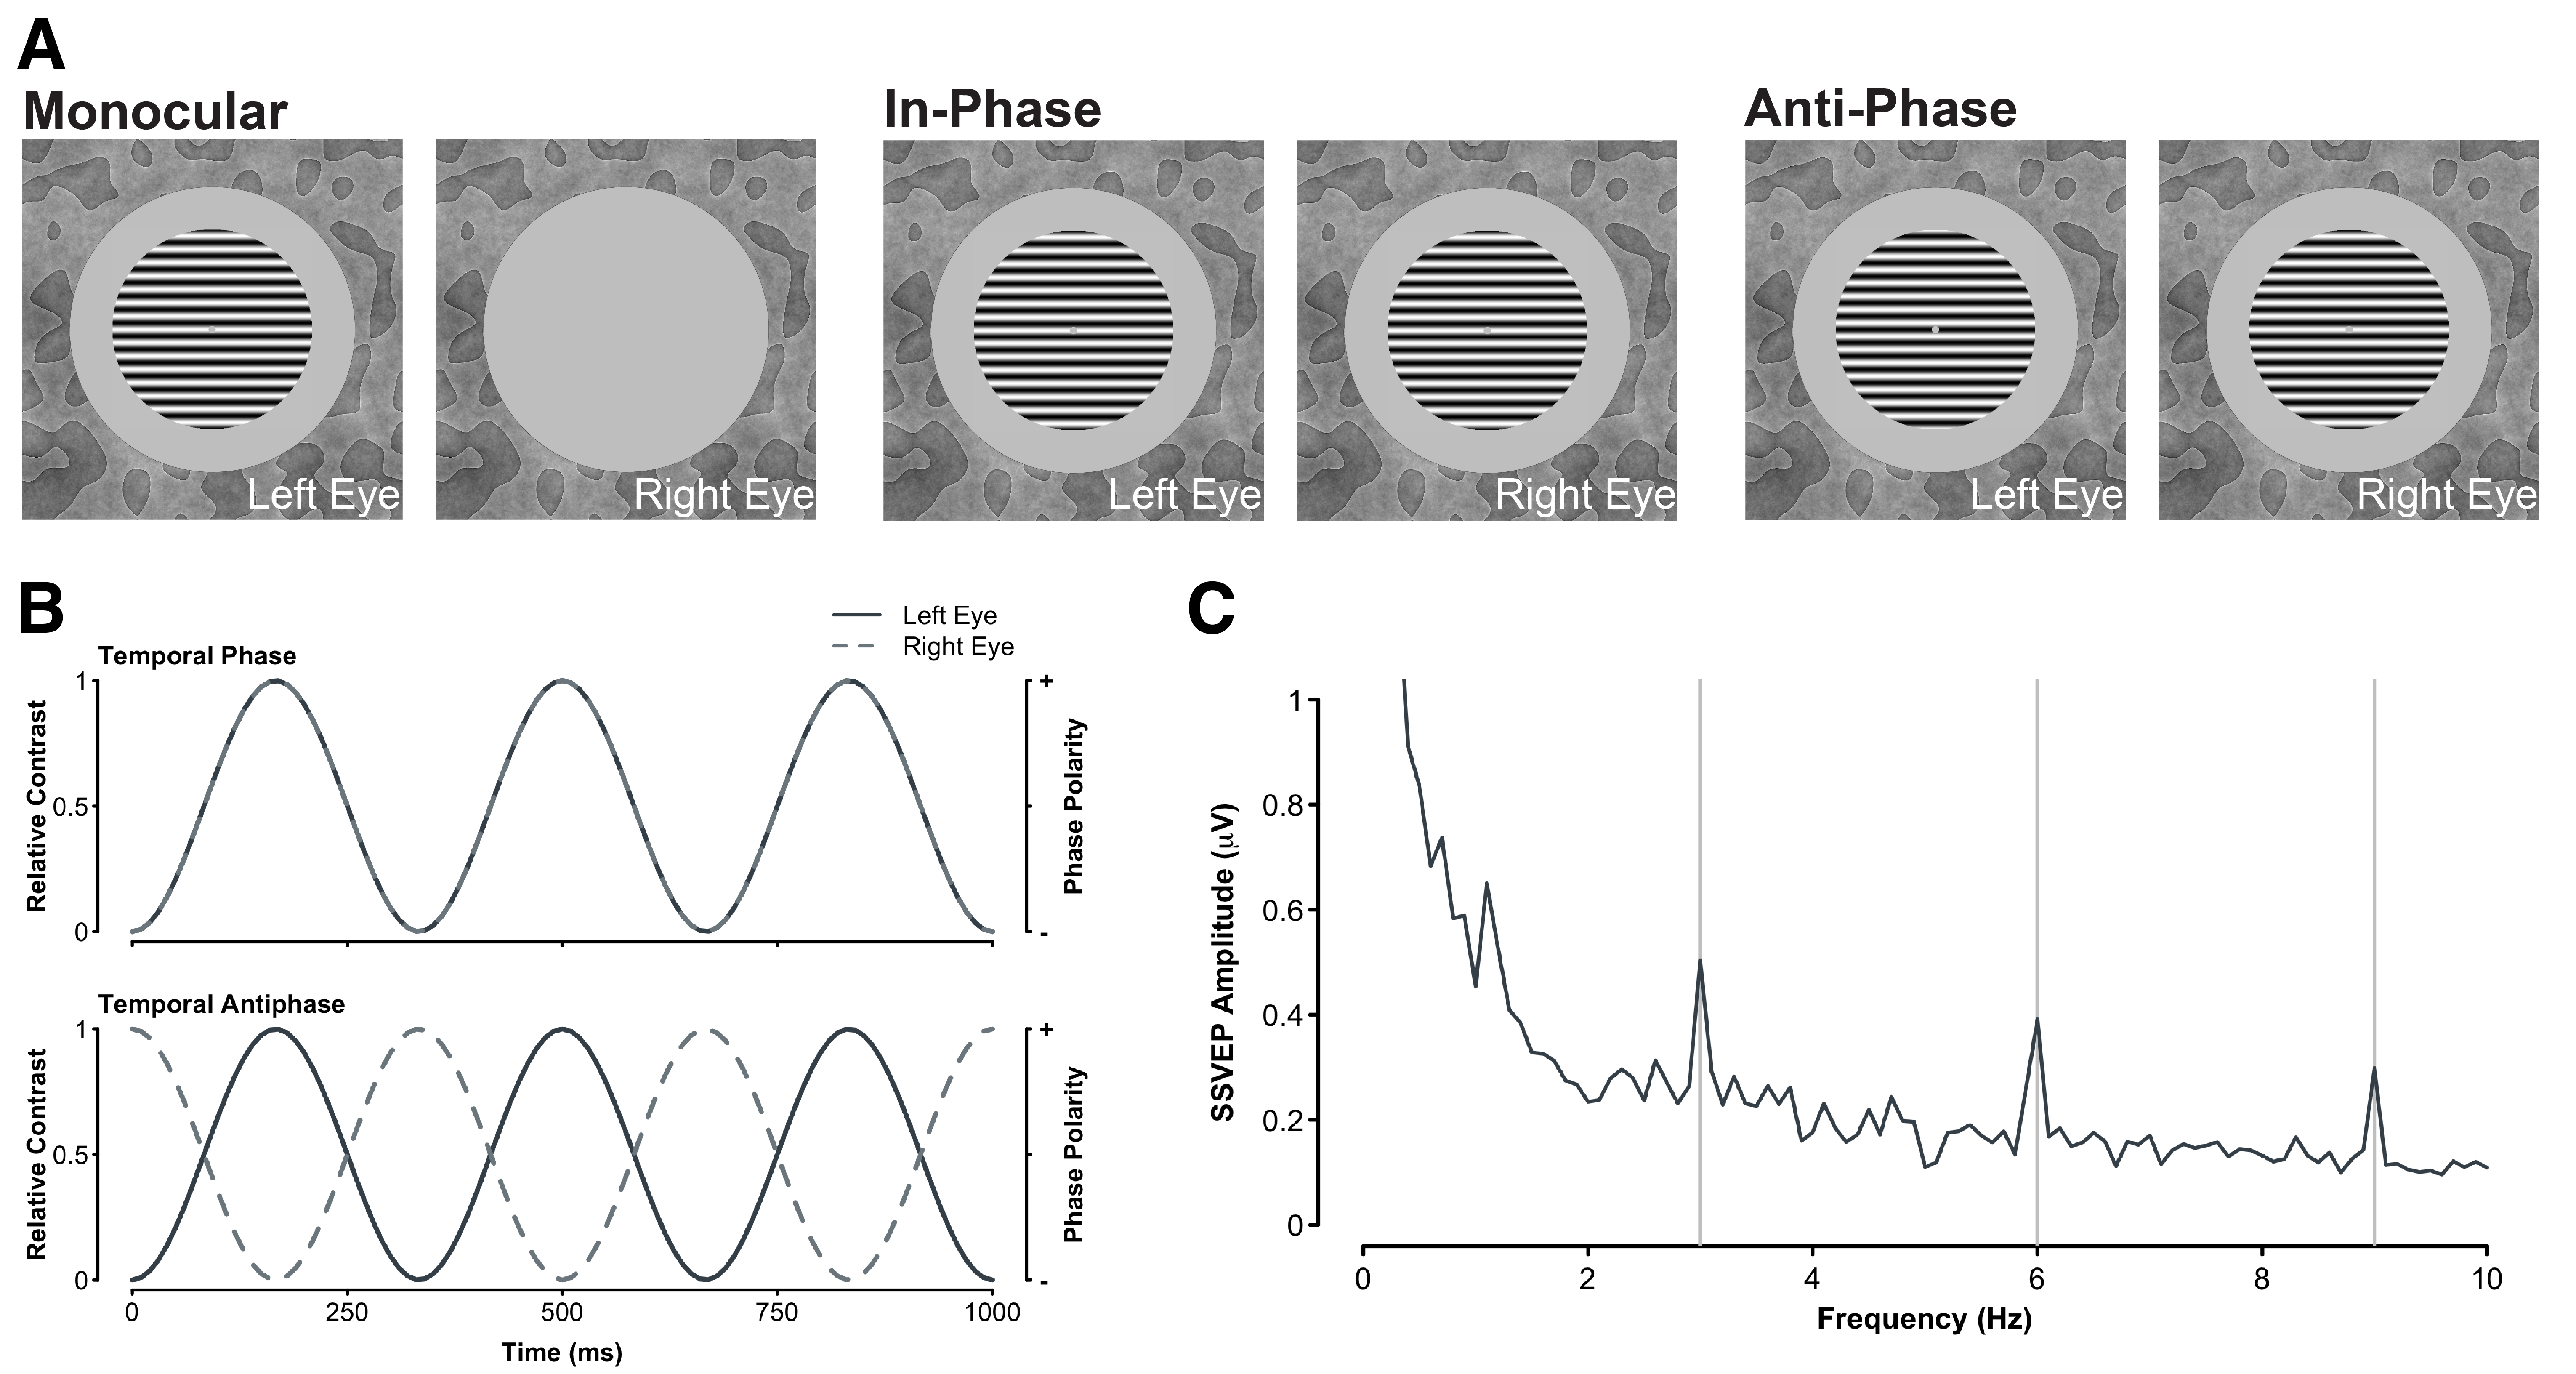
\includegraphics[keepaspectratio]{Figures/MethodsFigure.png}}

}

\caption{\label{fig-methodFigures}\textbf{A}. The spatial configuration
of stimuli presented to observers in our experiment. Monocular
conditions presented the sinusoidal grating to the left or right eye of
observers (counterbalanced) while the other eye was presented with a
gray screen set to mean luminance. Binocular conditions could be shown
with stimuli in spatial phase, whereby the phase of both sinusoidal
gratings was identical, or in spatial anti-phase, where the phase of the
sinusoidal gratings presented to each eye was opposite. The background
texture did not change throughout the trial to aid with binocular
fusion. \textbf{B}. The temporal configuration of our stimuli. To
generate SSVEPs, stimuli were contrast modulated in two ways: on/off
(left Y axis) or counterphase (right Y axis). The oscillatory pattern
could also be in phase (upper plot), where both stimuli were modulated
in the same manner, or in counterphase (lower plot), where as one
stimulus increased in contrast, the other decreased in contrast (or
increased in opposite polarity). \textbf{C}. Example SSVEPs generated
under binocular spatial and temporal in-phase viewing of stimuli for one
observer, with an average of four electrodes (\emph{Oz}, \emph{POz},
\emph{O1}, \emph{O2}) and 12 repetitions.}

\end{figure}%

Observer SSVEPs were measured with a single horizontal sinusoidal
grating that subtended 15\(^o\) of visual angle on the retina with a
spatial frequency of 3 cycles/\(^o\) of visual angle
(Figure~\ref{fig-methodFigures}A). Our experimental conditions modulated
the interocular spatial phase of stimuli
(Figure~\ref{fig-methodFigures}A). Under binocular viewing, the
sinusoidal gratings could be presented in spatial phase or spatial
anti-phase. When stimuli were presented in spatial phase, the aligned
sinusoidal gratings were identical in both eyes (\(\Delta \phi = 0\)).
The spatial anti-phase condition phase-shifted one of the sinusoidal
gratings by 180\(^o\) (\(\Delta \phi = \pi\)). Stimuli were also
modulated in their oscillatory pattern, which could be On/Off or
counterphase flicker at a frequency of 3Hz
(Figure~\ref{fig-methodFigures}B). Under On/Off contrast flicker, the
relative contrast of the gratings began at 0\%, increased smoothly to
100\% of the nominal maximum (100\% Michelson contrast), and then
returned to 0\% over 333 ms (i.e., one cycle). On/Off flicker will
generate SSVEPs at the fundamental frequency (3Hz) and its integer
harmonics (2F, 3F, 4F, see Figure~\ref{fig-methodFigures}C).
Counterphase flicker reversed the phase of the gratings at a frequency
of 3Hz. The contrast of the grating began at the relative maximum
(100\%), gradually decreased in contrast to 0\% of the relative maximum,
and then increased again to 100\% but in the opposite phase polarity.
Unlike On/Off flicker, counterphase flicker generates two nearly
identical transients per cycle and thus does not produce SSVEPs at the
fundamental frequency (3Hz) but only its even harmonics (Wade and Baker,
2025).

To aid with binocular fusion, stimuli were surrounded by a static
binocular texture presented beyond the central 19\(^o\) stimulus
aperture. These textures were constructed by first low-pass filtering a
white (amplitude \(\propto 1/f^0\)) noise pattern, dichotomizing its
output into a binary image and taking its phase spectrum. A second flat
(amplitude \(\propto 1/f^0\)) was adjusted by multiplying each spatial
frequency's amplitude coefficient by \(f^{-1}\) to generate a pink
amplitude spectrum (Hansen and Hess, 2006; Tadmor and Tolhurst, 1994).
The pink amplitude spectrum and the phase spectrum of the binary image
were rendered in the spatial domain by taking the inverse Fourier
transform, resulting in the pattern shown in
Figure~\ref{fig-methodFigures}A.

\subsection{Procedures}\label{procedures}

Steady-State Visually Evoked Potentials (SSVEPs) were recorded with
monocular and binocular stimulation using either on-off or counterphase
flicker at 3Hz. Across the eyes, binocular stimuli could be in spatial
and temporal phases, in temporal phase but spatial anti-phase, in
spatial phase but temporal anti-phase, or spatial and temporal
anti-phase (on-off flicker only). Stimuli presented in spatial and
temporal anti-phase under counterphase flicker are identical to stimuli
presented in spatial and temporal phase (and so we did not duplicate
this condition). Thus, this experiment was comprised of a total of nine
conditions - two monocular and seven binocular - which were each
repeated 12 times for a total of 108 trials. Stimulus presentation was
separated into four experimental blocks, each containing 27 trials. A
trial lasted 15 seconds; a grating stimulus flickered onscreen for 11
seconds, followed by a screen with its central 19\(^o\) set to mean
luminance for 4 seconds. Participants completed all 27 trials of an
experimental block in a single sequence (6.75 minutes) and were given
breaks between experimental blocks. The trial order was
pseudo-randomized on each block. Participants did not receive explicit
task instructions other than to fixate the marker in the center of the
display and blink only during the blank period between stimulus
presentations.

\subsection{SSVEP Analysis}\label{ssvep-analysis}

We used whole-head average referencing to normalize each electrode to
the mean signal of all 64 electrodes (for each sample point). The EEG
waveforms were Fourier transformed at each electrode for a 10-second
window, beginning one second after the stimulus onset to avoid onset
transients. The Fourier spectra were coherently averaged (i.e.,
retaining the phase information) across four occipital electrodes
(\emph{Oz}, \emph{POz}, \emph{O1} and \emph{O2}) and trial repetitions
(see Figure~\ref{fig-methodFigures}C). We then calculated
signal-to-noise ratios (SNRs) by dividing the absolute amplitude in the
signal bin (e.g., 3 Hz) by the mean of the absolute value of the ten
adjacent bins (\(\pm 0.5\) Hz in steps of 0.1 Hz). Given that
distributions of SNRs are inherently skewed, the median SNR was taken
across all participants; the median is a more robust descriptor of
central tendency in skewed distributions.

\section{Results}\label{results}

\begin{figure}

\centering{

\pandocbounded{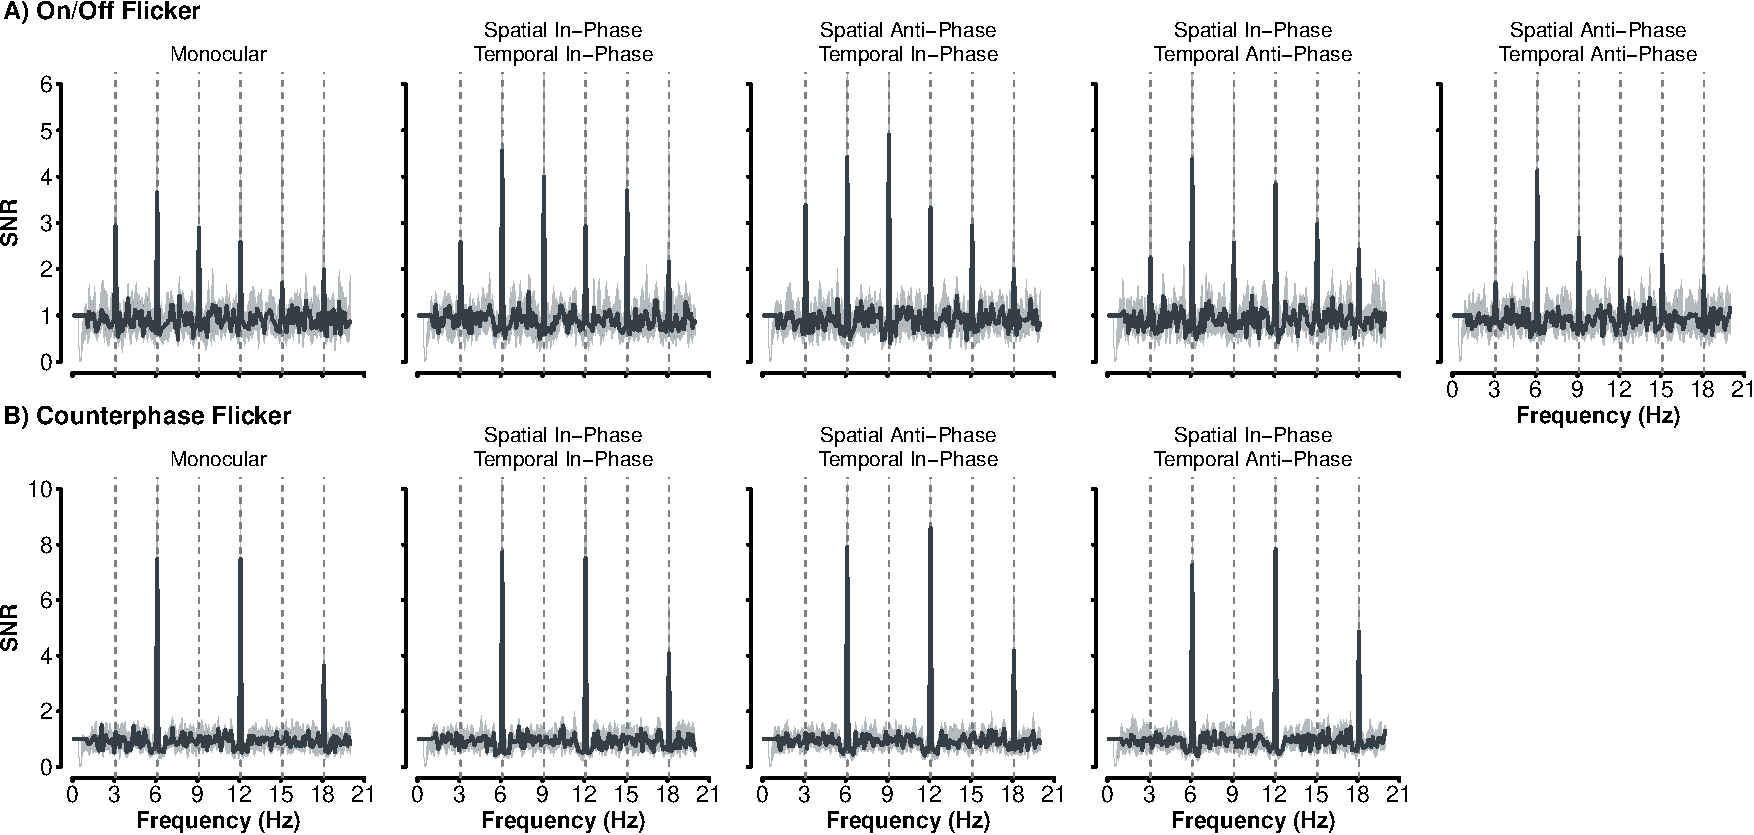
\includegraphics[keepaspectratio]{SSVEP_Phase_AntiPhase_paper_files/figure-pdf/fig-SNRData-1.pdf}}

}

\caption{\label{fig-SNRData}Cross-participant median SNRs for
frequencies up to 20Hz. SNRs generated by On/Off flicker are shown in
the top row (A), while those generated by counterphase flicker are shown
in the bottom row (B). The light gray area represents 95\% bootstrap
confidence intervals that were calculated by resampling (with
replacement) participant SNRs 2000 times.}

\end{figure}%

Figure~\ref{fig-SNRData} shows the cross-participant median SNR spectra
for all experimental conditions. Responses for all On/Off flicker
experimental conditions generated peaks at the fundamental frequency
(3Hz) and its harmonics (integer multiples of 3Hz). Similarly,
counterphase flicker produced responses at twice the flicker frequency
(6 Hz) and its harmonics. We assessed differences in SNR magnitude
across experimental conditions via a permutation test. A permutation
test allows for a non-parametric comparison of a statistic between two
experimental conditions. We first take the median difference between two
experimental conditions (i.e., the observed difference). A null
distribution is then constructed by combining SNR values from both
experimental conditions, and randomly sampled without replacement to
create two groups of sizes identical to their original, but with values
that are not associated with a particular experimental condition. The
median difference of the randomly sampled SNRs is then taken. This
process is repeated multiple times (e.g., \(N = 2000\)) to build a
distribution of median differences with no association of experimental
condition (i.e., a null-hypothesis distribution). The observed median
difference is then compared to this distribution, and the proportion of
scores greater (or less) than the observed difference represents the
\(p\) value associated with the test. When comparing SNRs at the
fundamental frequency (3Hz) for On/Off flicker, we find no statistically
significant difference in median SNR magnitude between experimental
conditions where stimuli were presented in temporal phase (see
Figure~\ref{fig-SNRComparison}). Monocular and binocular presentation
for stimuli presented in temporal phase resulted in a similar response
pattern under both On/Off and counterphase flicker modulations. This is
consistent with ocularity invariance; binocular and monocular stimuli
are judged equal in magnitude at high contrast (Baker et al., 2018;
Legge, 1984; Maehara and Goryo, 2005; Meese et al., 2006).

\begin{figure}

\centering{

\pandocbounded{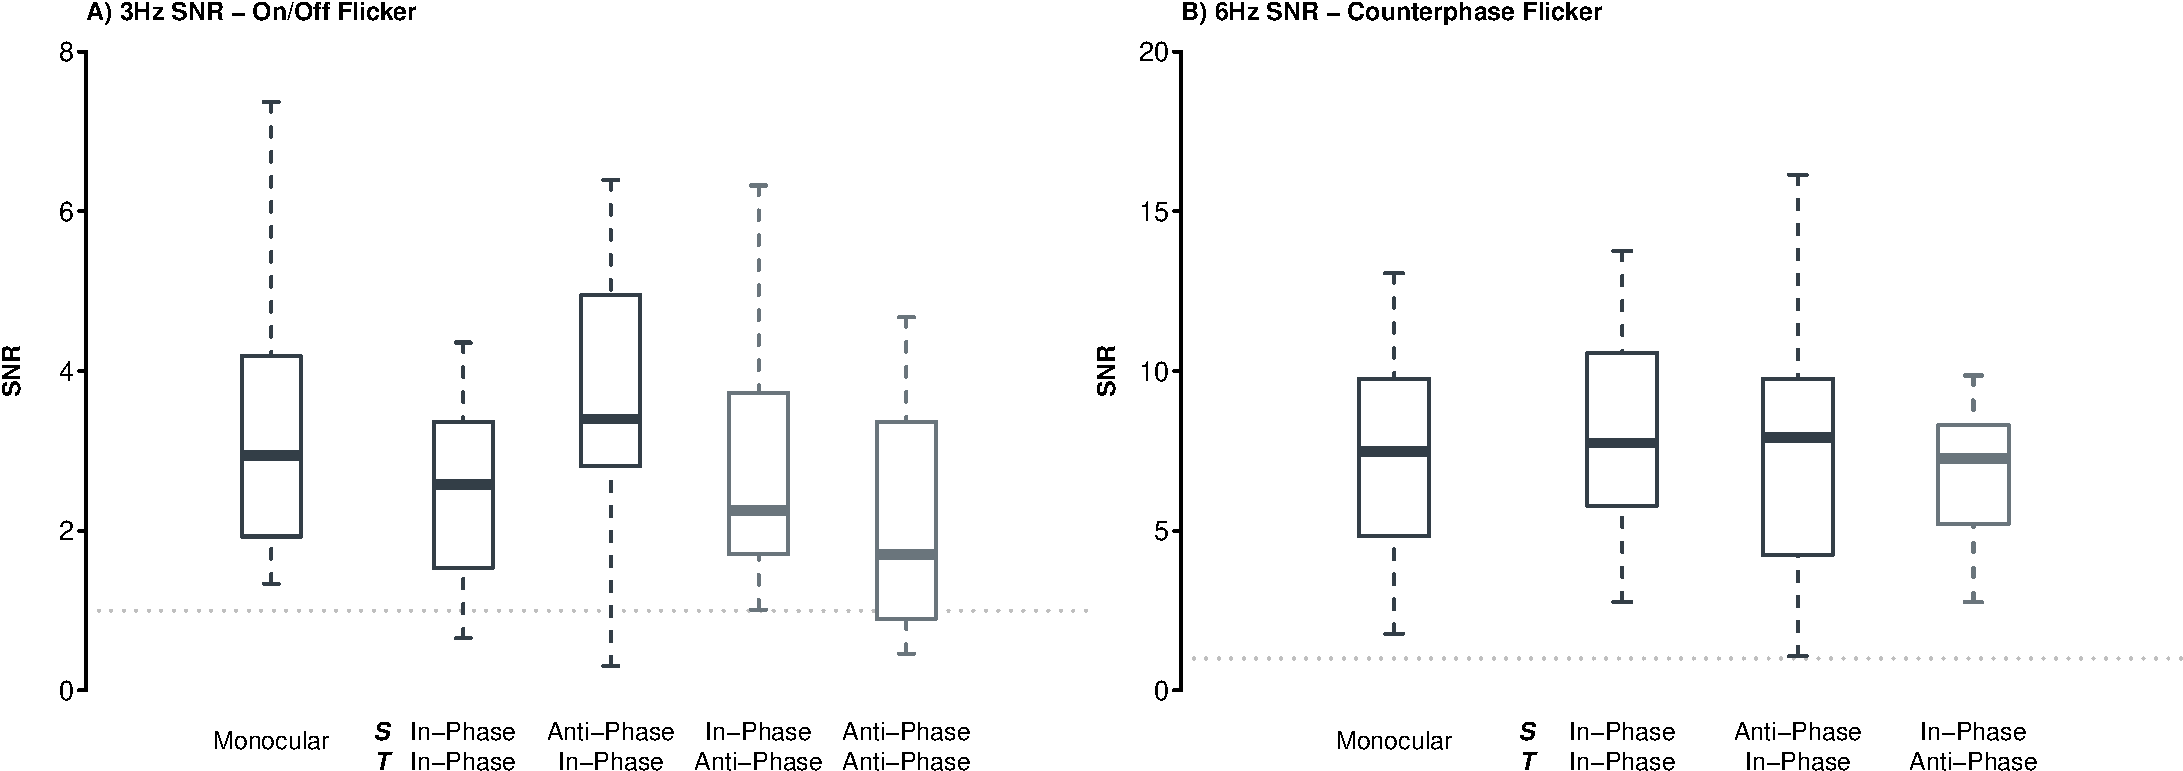
\includegraphics[keepaspectratio]{SSVEP_Phase_AntiPhase_paper_files/figure-pdf/fig-SNRComparison-1.pdf}}

}

\caption{\label{fig-SNRComparison}Boxplots of participant SNRs at the
fundamental frequency for each experimental condition in our study. A)
Boxplots represent the participant SNR at 3Hz. The median SNR is shown
by the thick line within the box, with the lower and upper border of the
box representing the first (25\%) and third (75\%) quartile of the SNR
distribution. Dashed lines show the lower and upper whisker limits,
which are calculated as 1.5 times the interquartile range (distance
between the third and first quartile). Boxplots for the binocular
conditions have labels for their spatial (S) and temporal (T) phase
relationships. Experimental conditions where stimuli are presented in
temporal anti-phase are shown in a lighter gray. B) As in A, boxplots
show participant SNRs at 6Hz, the fundamental frequency for counterphase
flicker. In both graphs, the dashed line represents an SNR of 1.0.}

\end{figure}%

Changing the phase relationships of stimuli under On/Off flicker had
some interesting impacts on the fundamental frequency
(Figure~\ref{fig-SNRComparison}A). Stimuli presented in spatial phase
and temporal anti-phase generated smaller SNRs (median\(_{\text{SNR}}\)
= 2.25) than stimuli presented in spatial anti-phase and temporal phase
(median\(_\text{SNR}\) = 3.40, \(p\) = .047). The reduction in the
amplitude relative to stimuli in spatial anti-phase and temporal phase
was also observed for stimuli in temporal and spatial anti-phase
(median\(_\text{SNR}\) = 1.70; \(p\) = .023). No other statistically
significant difference in median SNRs were observed for all counterphase
flicker conditions or the other harmonics for On/Off flicker (all \(p\)
values were greater than .05). While the median SNRs under On/Off
flicker shown in temporal anti-phase were reduced in comparison to other
conditions, both the spatial in phase temporal anti-phase condition
(\(p < .001\)) and the spatial and temporal anti-phase conditions
(\(p = .004\)) had median SNR values that were statistically
significantly greater than 1.0. The presence of a 3Hz response for
binocular stimuli presented in temporal anti-phase indicates that
monocular responses remain and contribute to the SSVEP, as these
conditions generate two transients per cycle and a purely binocular
signal would only generate responses at 6Hz (Blake et al., 1981;
Georgeson et al., 2016; Moulden, 1980).

\subsection{Modelling}\label{modelling}

The perception of stimulus contrast across eyes is well-explained by
psychophysical models that process input contrast in two sequential
contrast gain control stages interposed by binocular summation (Baker et
al., 2008, 2007a, 2007b; Baker and Meese, 2007; Meese et al., 2006).
This simple, yet powerful, family of models not only captures
behavioural data well, but can also explain neural responses to
binocular and dichoptic stimuli (Baker and Wade, 2017; Lygo et al.,
2021; Richard et al., 2018). Our SSVEP results show the expected pattern
of binocular combination for stimuli presented at high contrast (i.e.,
ocularity invariance) but also intriguing effects that are likely
explainable by the most recent extension of the two-stage contrast gain
control model, as defined in Georgeson et al. (2016). To explore the
architecture required to describe our effects adequately, we
progressively increase the complexity of binocular combination beginning
with a wrong model (i.e., linear combination) and building up to a
multi-channel model with monocular, binocular and phase-selective
pathways (Figure~\ref{fig-modelDiagram}).

\begin{figure}

\centering{

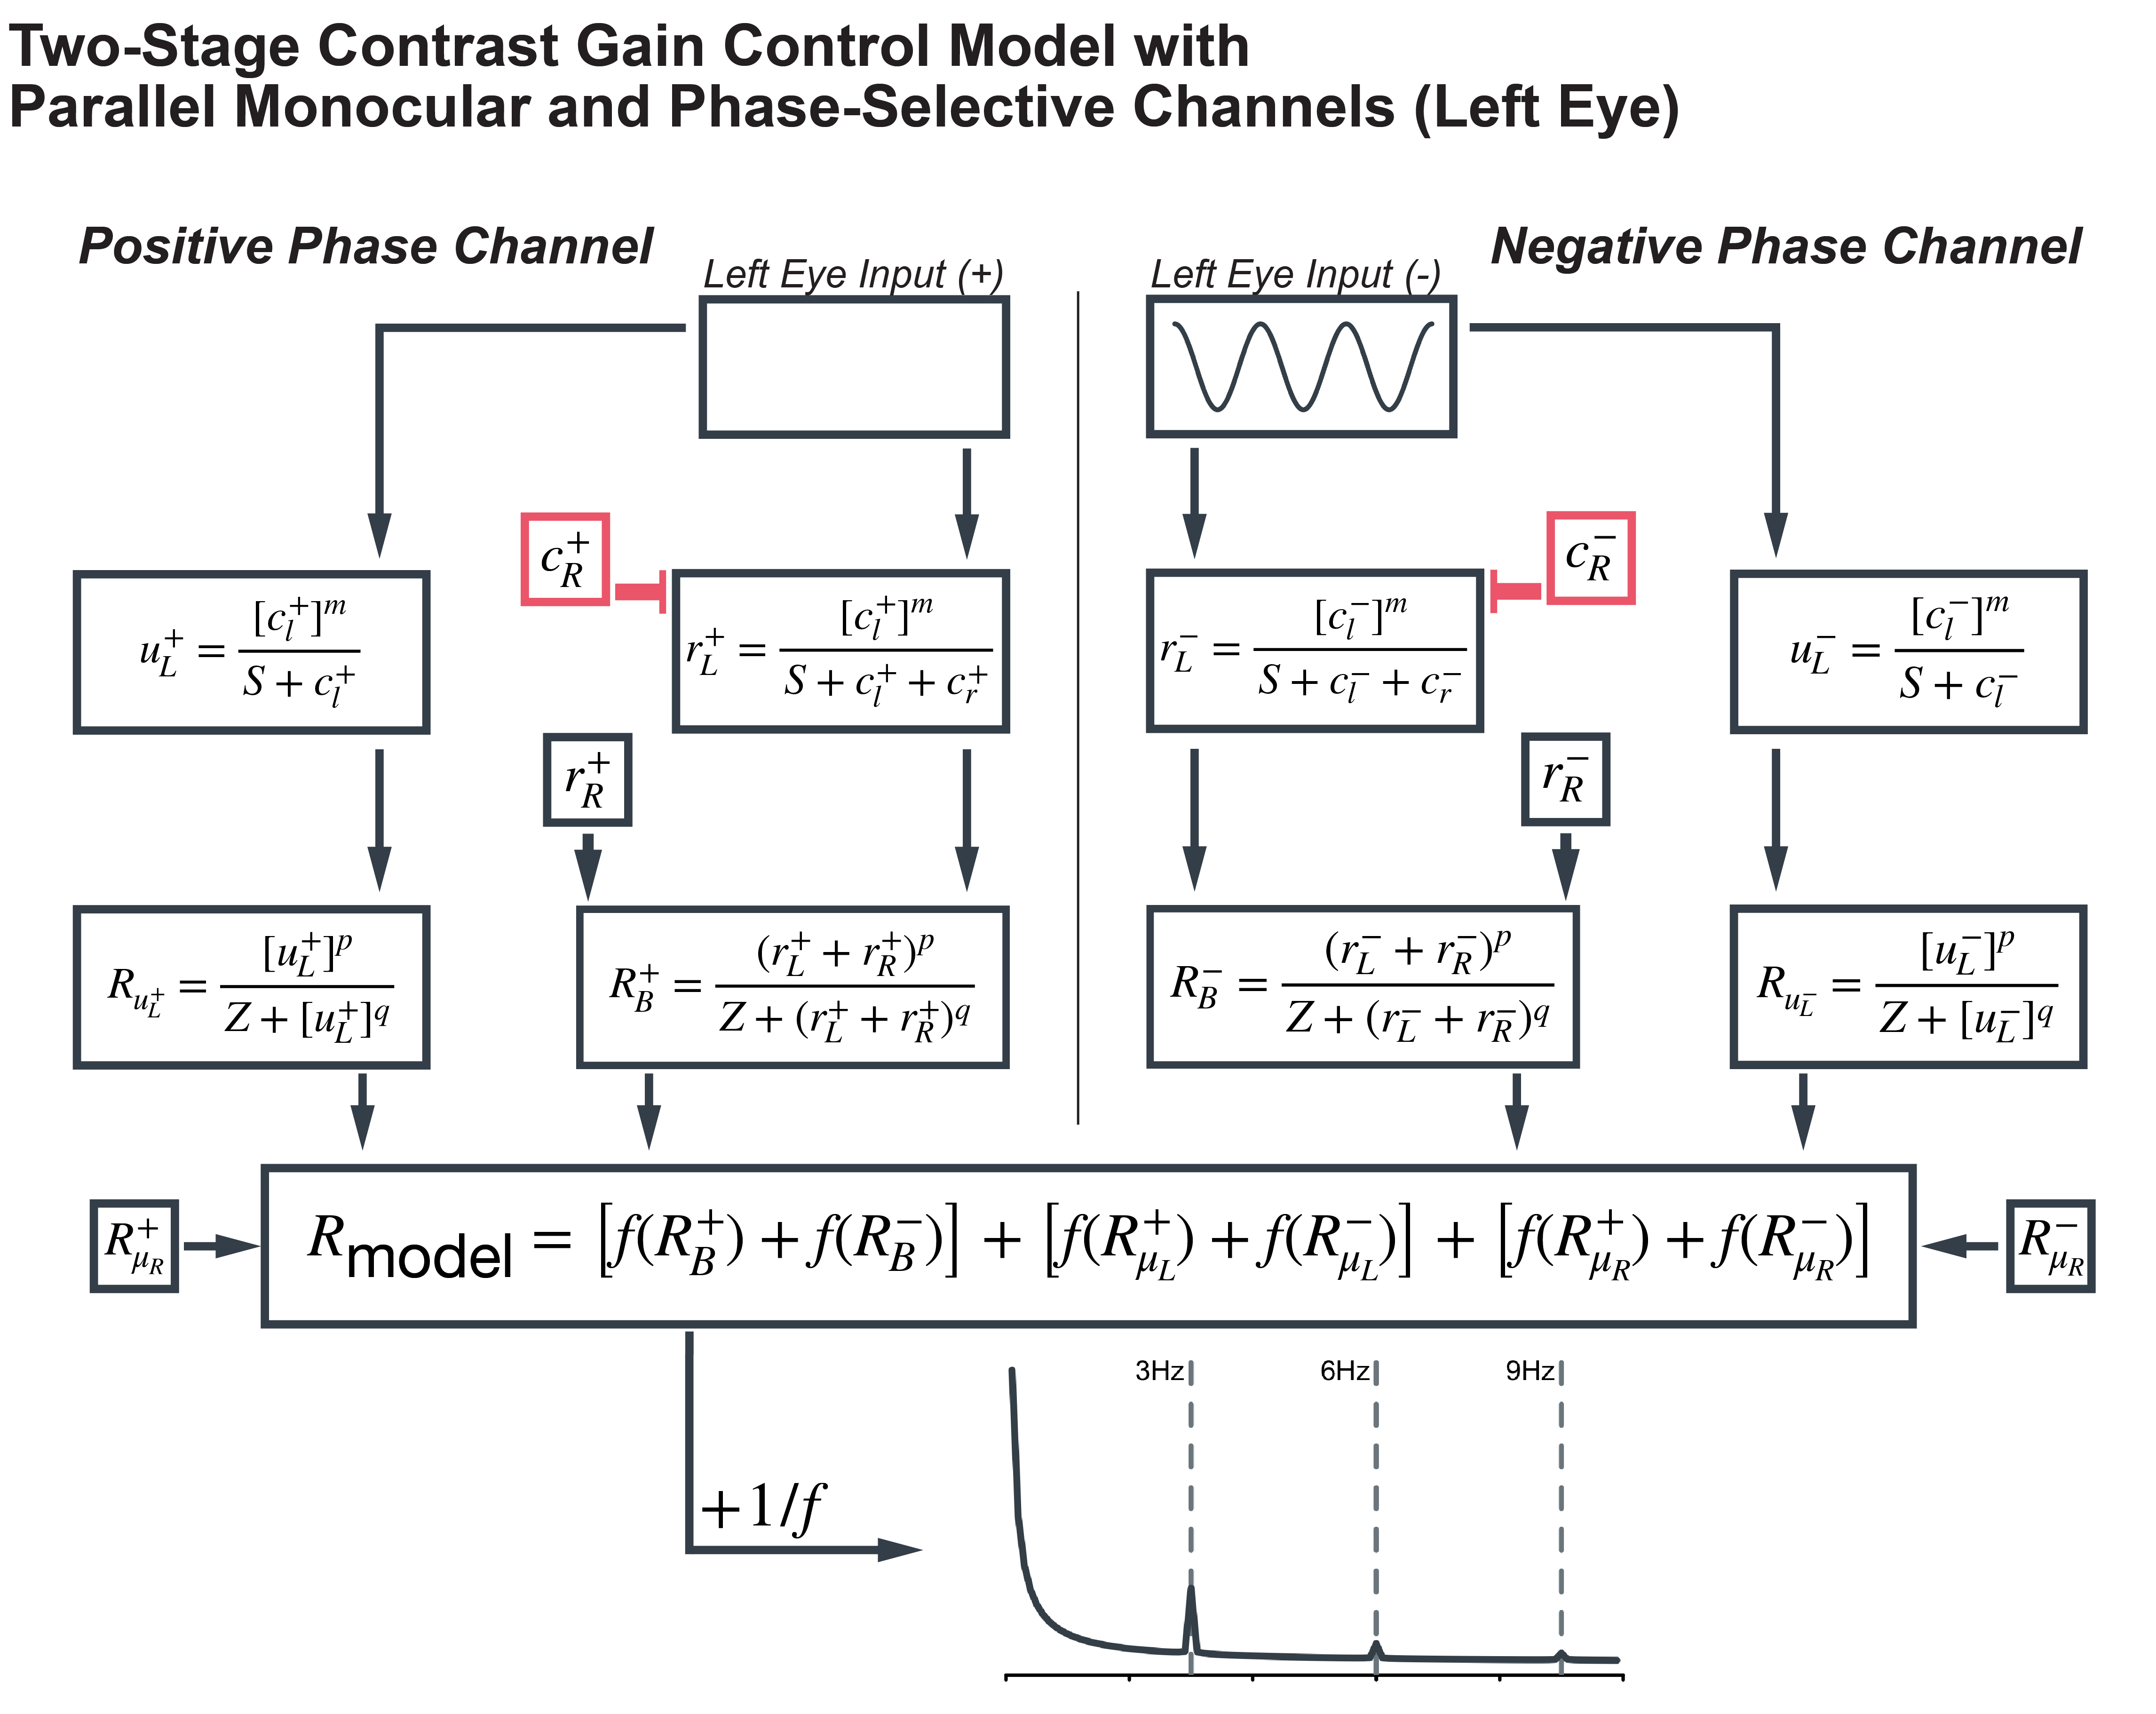
\includegraphics[width=0.8\linewidth,height=\textheight,keepaspectratio]{Figures/FullModel.png}

}

\caption{\label{fig-modelDiagram}The multi-channel variant of the
two-stage contrast gain control model. This diagram shows the channels
for the left eye. Contributions from the right eye (\(c^+_R\) and
\(r^+_R\)) to the binocular channels are shown in small boxes. Unlike
the model defined by Georgeson et al. (2016), responses from the
parallel monocular channels are added to those of the binocular channels
before signal selection for phase-selective channels. This change
accounts for methodological differences when fitting neuroimaging data.
To fit the final response of the model, \(R\), was Fast Fourier
Transformed, and a pink noise spectrum was added to allow for a
comparable calculation of model SNRs as is done with human data.}

\end{figure}%

The architecture of the models explored differs, but all received the
same input and had their final outputs processed identically. The input
to all models was a 3 Hz sine wave, adjusted to accurately represent the
various experimental conditions of this study (see
Figure~\ref{fig-methodFigures}). For example, stimuli presented with
On/Off flicker in temporal anti-phase had the left eye input generated
by the following equation,
\begin{equation}\phantomsection\label{eq-stimInput2L}{
c_L = A * (\cos(2 \pi ft)+1)/2,
}\end{equation} while the right eye input would be defined as,
\begin{equation}\phantomsection\label{eq-stimInput2R}{
c_R = A * (-\cos(2 \pi ft)+1)/2.
}\end{equation} \(A\) represents stimulus contrast (amplitude), \(f\)
the temporal flicker frequency (i.e., 3 Hz), and \(t\) time in
milliseconds. The input to the other eye (\(c_R\)) is phase shifted by
180\(^o\), which can be accomplished using the negative cosine function
(\(-cos\)). Finally, sine waves are rectified to range between 0 and 1
to represent the relative contrast presented to observers. The same
experimental condition with counterphase flicker has the following
sinusoidal profile for the left eye,
\begin{equation}\phantomsection\label{eq-stimInput3L}{
c_L = A * [\cos(2 \pi ft)]_+
}\end{equation} and for the right eye,
\begin{equation}\phantomsection\label{eq-stimInput3R}{
c_R = A * [-\cos(2 \pi ft)]_+.
}\end{equation} These profiles are identical to the On/Off flicker, but
the sine waves are half-wave rectified to represent the counterphase
oscillation. To fit model outputs (rectified sine waves) to observer
data, the final response of the models was Fast Fourier Transformed, and
a pink noise spectrum was added to the Fourier amplitude,
\(|FFT(R_\text{model})|+1/f\), before calculating model SNRs. All models
developed in this study were fit by minimizing the sum of squared errors
between the model output and the observer median SNRs for the first 6
SSVEP components (3Hz, 6Hz, 9Hz, 12Hz, 15Hz, and 18Hz).

\subsubsection{Evidently wrong models}\label{evidently-wrong-models}

As a first step in defining the necessary architecture to capture our
results, we built wrong models with no monocular stage or phase
selectivity. The first is a purely linear summation model of binocular
combination, \begin{equation}\phantomsection\label{eq-linearSumModel}{
R_B = c_L+c_R,
}\end{equation} the binocular response (\(R_B\)) is the sum of the
monocular inputs. The fits of the linear summation model are shown in
Figure~\ref{fig-badModels1} and its performance metrics in
Table~\ref{tbl-R2Table}. For On/Off flicker, the linear summation model
only generates responses at the fundamental frequency (3Hz) that grossly
overestimate observer SNRs. This is expected as this model lacks the
rectification and non-linearities required to generate responses at the
harmonics (Regan and Regan, 1988; Wade and Baker, 2025). In a linear
sum, stimuli presented under On/Off flicker in temporal anti-phase
cancel each other, and thus the model generates no response. The model
does generate responses at the fundamental and harmonics of the
counterphase flicker condition (Figure~\ref{fig-badModels1}B), but this
is attributable to the input's rectification (the half-wave
rectification applied to the input;
Equation~\ref{eq-stimInput3L}, Equation~\ref{eq-stimInput3R}) and not
the model architecture.

\begin{longtable}[]{@{}
  >{\raggedright\arraybackslash}p{(\linewidth - 6\tabcolsep) * \real{0.6104}}
  >{\centering\arraybackslash}p{(\linewidth - 6\tabcolsep) * \real{0.1299}}
  >{\centering\arraybackslash}p{(\linewidth - 6\tabcolsep) * \real{0.1299}}
  >{\centering\arraybackslash}p{(\linewidth - 6\tabcolsep) * \real{0.1299}}@{}}
\toprule\noalign{}
\begin{minipage}[b]{\linewidth}\raggedright
Model
\end{minipage} & \begin{minipage}[b]{\linewidth}\centering
\(R^2\)
\end{minipage} & \begin{minipage}[b]{\linewidth}\centering
RMSE
\end{minipage} & \begin{minipage}[b]{\linewidth}\centering
AIC
\end{minipage} \\
\midrule\noalign{}
\endfirsthead
\toprule\noalign{}
\begin{minipage}[b]{\linewidth}\raggedright
Model
\end{minipage} & \begin{minipage}[b]{\linewidth}\centering
\(R^2\)
\end{minipage} & \begin{minipage}[b]{\linewidth}\centering
RMSE
\end{minipage} & \begin{minipage}[b]{\linewidth}\centering
AIC
\end{minipage} \\
\midrule\noalign{}
\endhead
\bottomrule\noalign{}
\tabularnewline
\caption{Goodness-of-fit metrics for all models compared in this study.
Errors in predictions for the linear sum model were too large to
calculate \(R^2\). RMSE is the Root Mean Square error and AIC is the
Aikaike Information Criterion.}\label{tbl-R2Table}\tabularnewline
\endlastfoot
Linear sum & - & 3.234 & 281.99 \\
Linear sum, with Rectification & 0.575 & 1.405 & 197.95 \\
Two-Stage, no interocular interactions & 0.822 & 0.908 & 154.86 \\
Two-Stage, with interocular interactions & 0.81 & 0.94 & 158.62 \\
Two-Stage with parallel monocular channels & 0.877 & 0.756 & 135.1 \\
Two-Stage with phase-selective channels \& monocular channels & 0.876 &
0.759 & 135.39 \\
\end{longtable}

Responses of neurons to contrast in the visual system are well-modeled
by a saturating non-linearity: as contrast increases, the magnitude of
responses saturates (the increase in response per unit contrast
decreases at higher contrast values; Heeger (1992)). The saturating
non-linearity can be modeled in different ways, but generally contains a
divisive suppression and an exponentiation of the excitatory and
inhibitory inputs. The inclusion of suppression can aid the model in
better capturing the magnitude of responses in our observers while
exponents introduces the non-linearities required to generate responses
at the harmonic frequencies. Thus, the next increment in our model
complexity defines the binocular response as the contrast gain control
equation \begin{equation}\phantomsection\label{eq-firstBinocSum}{
R_B = \frac{(c_L+c_R)^p}{Z+(c_L+c_R)^q},
}\end{equation} where the binocular response of the model (\(R_B\)) is
defined as the sum of monocular inputs (\(c_L\) and \(c_R\)) raised to
the power \(p\) normalized by the sum of monocular inputs raised to the
power \(q\) and where (\(p\) \textgreater{} \(q\)). The parameter Z
prevents division by zero. The model can now generate responses at the
harmonic frequencies for stimuli presented in temporal phase under
On/Off flicker (see Figure~\ref{fig-badModels1} and
Table~\ref{tbl-R2Table}). While this model iteration improves on the
fits, it nevertheless struggles to fit SNR values at the fundamental
frequency (3Hz) and is, as with the linear summation model, incapable of
generating responses to stimuli presented with On/Off flicker in
temporal anti-phase; the linear sum of stimuli presented in temporal
anti-phase will always return zero. The model, therefore, still lacks
the necessary architecture to adequately define neural responses to our
stimuli.

\begin{figure}

\centering{

\pandocbounded{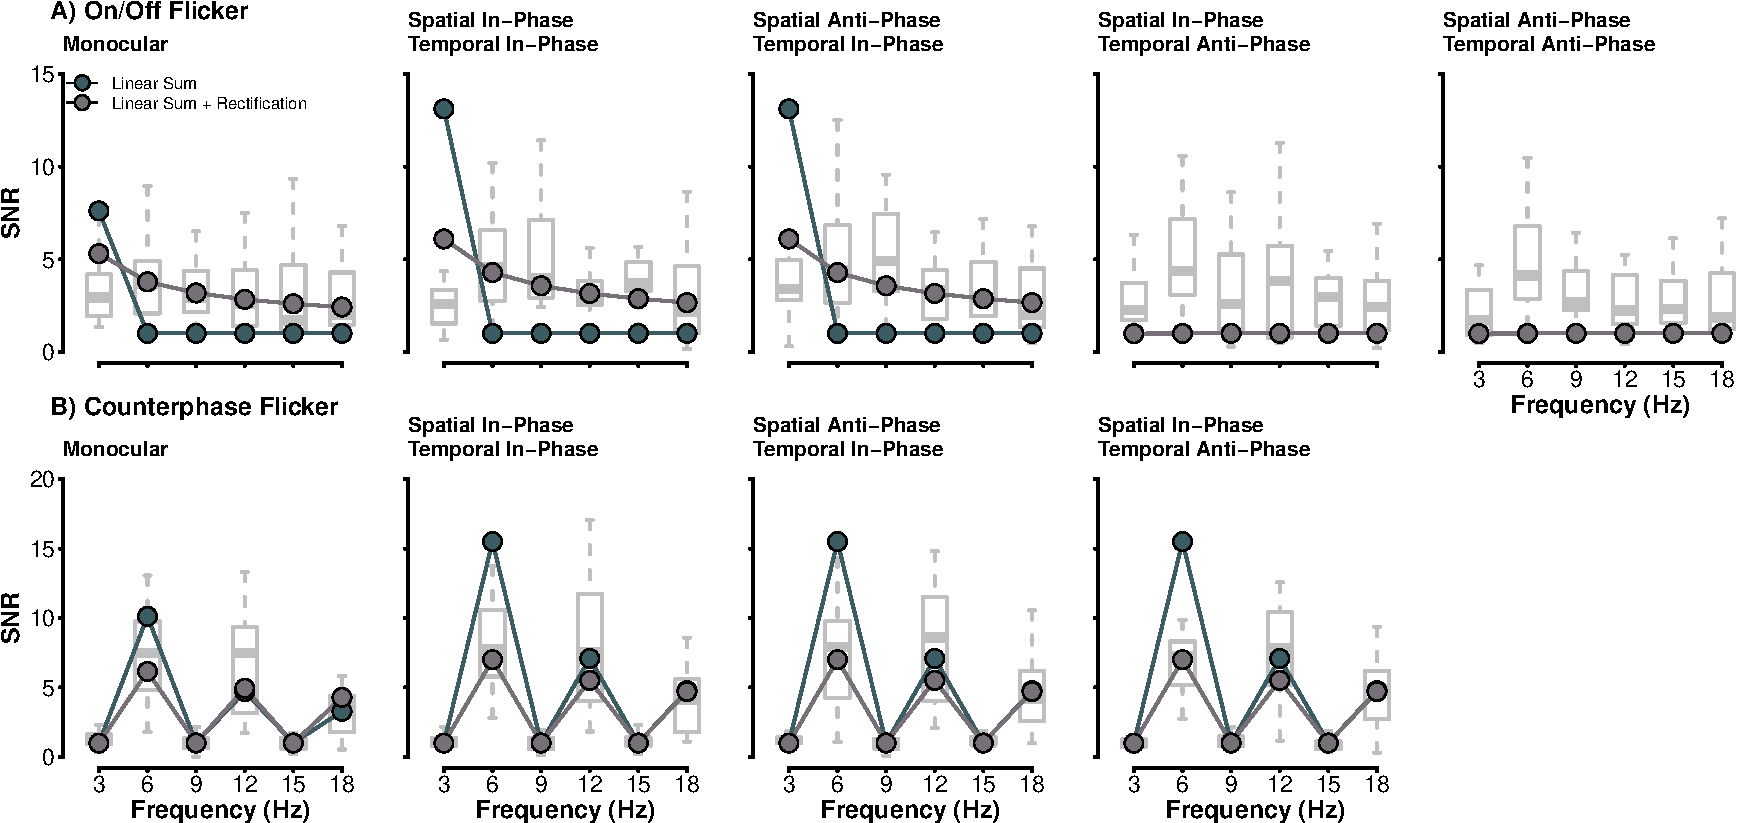
\includegraphics[keepaspectratio]{SSVEP_Phase_AntiPhase_paper_files/figure-pdf/fig-badModels1-1.pdf}}

}

\caption{\label{fig-badModels1}Fits of the linear sum (green) and the
rectified linear sum (brown) models. Boxplots behind model responses
show the distribution of observer SNRs. Model SNRs were fit to the
median SNR of observers, which is represented by the thicker line within
the box.}

\end{figure}%

\subsubsection{The Two-Stage Contrast Gain Control
Model}\label{the-two-stage-contrast-gain-control-model}

The simple models described above could not accurately represent the
observer SSVEPs we recorded. They overestimated SNRs at the fundamental
frequency and failed to generate responses for stimuli presented in
temporal anti-phase with On/Off flicker. A potential refinement to the
model is add a monocular transducer prior to binocular combination Baker
et al. (2018). The architecture of this model now begins with a
monocular stage
\begin{equation}\phantomsection\label{eq-firstStageofTwoNoInter}{
r_L = \frac{c_L^m}{S + c_L}, \qquad r_R = \frac{c_R^m}{S + c_R}
}\end{equation} where a non-linearity (\(m\)) is applied to the
monocular inputs (\(c_L\) and \(c_R\)) in addition to self-suppression.
The outputs of the monocular stage are then fed into a binocular stage
that undergoes a second contrast gain control,
\begin{equation}\phantomsection\label{eq-binocComb}{
R_{B} = \frac{(r_L+r_R)^p}{Z+(r_L+r_R)^q}.
}\end{equation} In this model variant, \(m\) is the monocular excitatory
component and determines the extent of summation at detection threshold,
moderated by the suppressive term. In the second stage, \(p > q\) as
with Equation~\ref{eq-firstBinocSum}, which is necessary to capture the
facilitative effects of dichoptic masking (Meese et al., 2006). We can
strengthen the normalization of the monocular input by adding
interocular suppression and replacing
Equation~\ref{eq-firstStageofTwoNoInter} (the first stage) with
\begin{equation}\phantomsection\label{eq-firstStageofTwo}{
r_{L} = \frac{c_L^m}{S + c_L + c_R}, \qquad r_R = \frac{c_R^m}{S + c_R + c_L}.
}\end{equation} This model iteration is identical to the two-stage
contrast gain control model defined by Meese et al. (2006).

\begin{figure}

\centering{

\pandocbounded{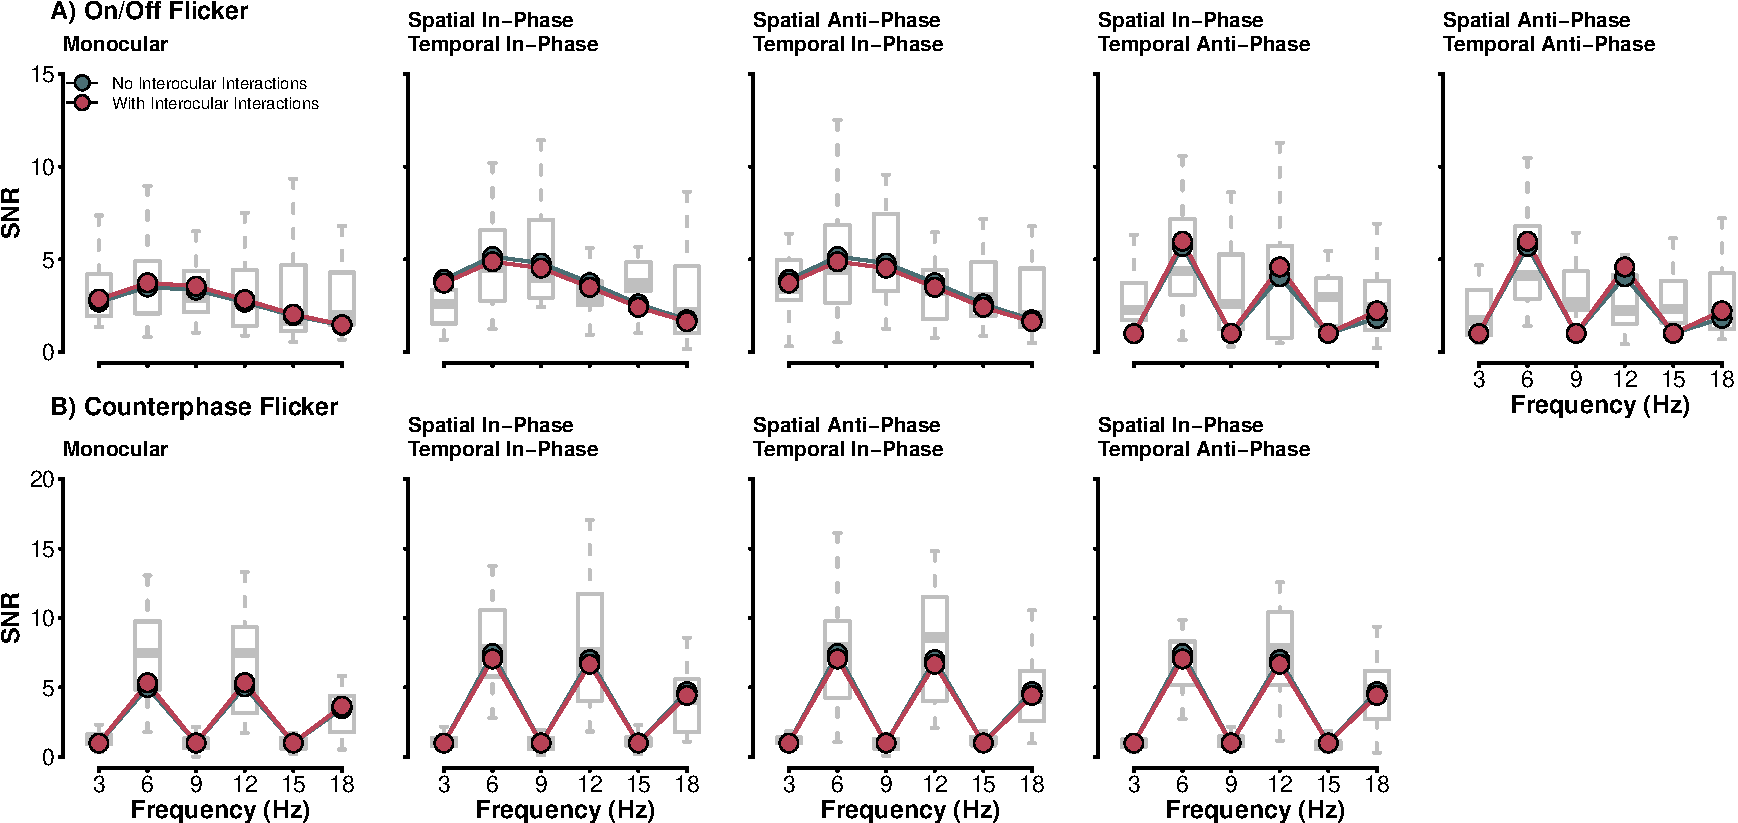
\includegraphics[keepaspectratio]{SSVEP_Phase_AntiPhase_paper_files/figure-pdf/fig-betterModels-1.pdf}}

}

\caption{\label{fig-betterModels}Fits of the two-stage contrast gain
control model without (green) and with (red) interocular suppression.
Boxplots behind model responses show the distribution of observer SNRs.
Model SNRs were fit to the median SNR of observers, which is represented
by the thicker line within the box.}

\end{figure}%

The fits of both model variants, with and without interocular
suppression, are shown in Figure~\ref{fig-betterModels}. The difference
in their quality is negligible (see Table~\ref{tbl-R2Table}) as both
describe most experimental conditions well. The addition of the
monocular transducer enables the model to fit observer SNRs at the
fundamental frequency for stimuli presented in temporal phase under
On/Off flicker and importantly, it now generates responses for stimuli
presented in temporal anti-phase. The transduced monocular inputs no
longer cancel each other at the binocular stage. While the model can
generate responses to temporal anti-phase stimuli, it only does so at
the even-harmonics (2F-6Hz, 4F-12Hz, and 6F-18Hz) of the SSVEP spectrum.
This is to be expected as the model can only generate binocular
responses; it does not preserve monocular responses beyond the first
stage. As the two rectified sine waves are in anti-phase, their sum will
generate a new waveform with frequencies at twice the frequency of the
original (6Hz) and its integer harmonics (2F-12Hz and 3F-18Hz; see
\textbf{?@fig-sumDiagram} \textbf{maybe in the appendix?}). The
responses at the fundamental frequency (3Hz) and its odd integer
harmonics (3F - 9Hz, 5F - 15Hz) of our observers cannot be explained by
an architecture with a purely binocular output. Next, we explore methods
of preserving the monocular signal in an effort to explain observer
responses to stimuli presented in temporal anti-phase.

\subsubsection{Parallel Monocular and Phase-Selective
Channels}\label{parallel-monocular-and-phase-selective-channels}

Observer SNRs for stimuli presented in temporal anti-phase contain a
binocular and monocular response to stimuli. To preserve the monocular
response in the modelling, we add parallel monocular channels to the
two-stage contrast gain control model, similar to Georgeson et al.
(2016). These channels are fully monocular and do not include
interocular suppression,
\begin{equation}\phantomsection\label{eq-monocFirstStage}{
\mu_L = \frac{C_L^m}{S + C_L}, \qquad  \mu_R = \frac{C_R^m}{S + C_R}.
}\end{equation} In this equation, \(\mu_L\) is the output of the first
stage of the monocular channel for the left eye, and \(\mu_R\) is that
of the right eye. The excitatory exponent \(m\) is identical to that in
the channels that include binocular interaction (see
Equation~\ref{eq-firstStageofTwo}). The output of the monocular channels
undergoes a second contrast gain control stage identical to that of the
binocular channel,
\begin{equation}\phantomsection\label{eq-monocSecondStage}{
R_{\mu_L} = \frac{\mu_L^p}{Z + \mu_L^q}, \qquad  R_{\mu_R} = \frac{\mu_R^p}{Z + \mu_R^q}.
}\end{equation} \(R_{\mu_L}\) and \(R_{\mu_R}\) represent the final
responses of the left and right monocular channels. No additional free
parameters are included in the model with parallel monocular channels;
the parameters \(m\), \(p\), \(q\), \(S\) and \(Z\) used to define the
monocular channel responses are identical to those of the binocular
channels.

\textbf{The addition of monocular channels poses an interesting problem
in generating the SSVEPs from the model. The final stage of this model
has three channel responses: monocular left (\(R_L\)), monocular right
(\(R_R\)), and binocular (\(R_B\)). In behavioural variants of this
model (Georgeson et al., 2016), cue selection is implemented as a MAX
rule, as a Minkowski sum with a very large (\(\approx 30\)) exponent.
This method of signal combination was not appropriate for SSVEP data, as
the signal we record is pool of neural responses at the scalp better
defined by a linear combination of the binocular and monocular signals,}
\begin{equation}\phantomsection\label{eq-binocMonocComb}{  
R_\text{model}=R_B+R_{\mu_L}+R_{\mu_R}.
}\end{equation}

In our model fits, we use the monocular response from the left eye
(\(R_{\mu_L}\)) to add to the binocular channel. {[}Not sure I
understand this bit - why not add both monocular channels?{]} Adding
parallel monocular channels to the two-stage contrast gain control model
significantly improved the fit of our observer data
(Figure~\ref{fig-bestModels}). With the monocular response preserved,
the model can now generate SSVEPs at the fundamental frequency and
odd-harmonics necessary to capture observer data for stimuli presented
in temporal anti-phase under On/Off flicker (see
Table~\ref{tbl-R2Table}). Thus, monocular responses to binocular stimuli
are preserved along the processing pipeline and can be recorded in the
SSVEPs of observers.

\begin{figure}

\centering{

\pandocbounded{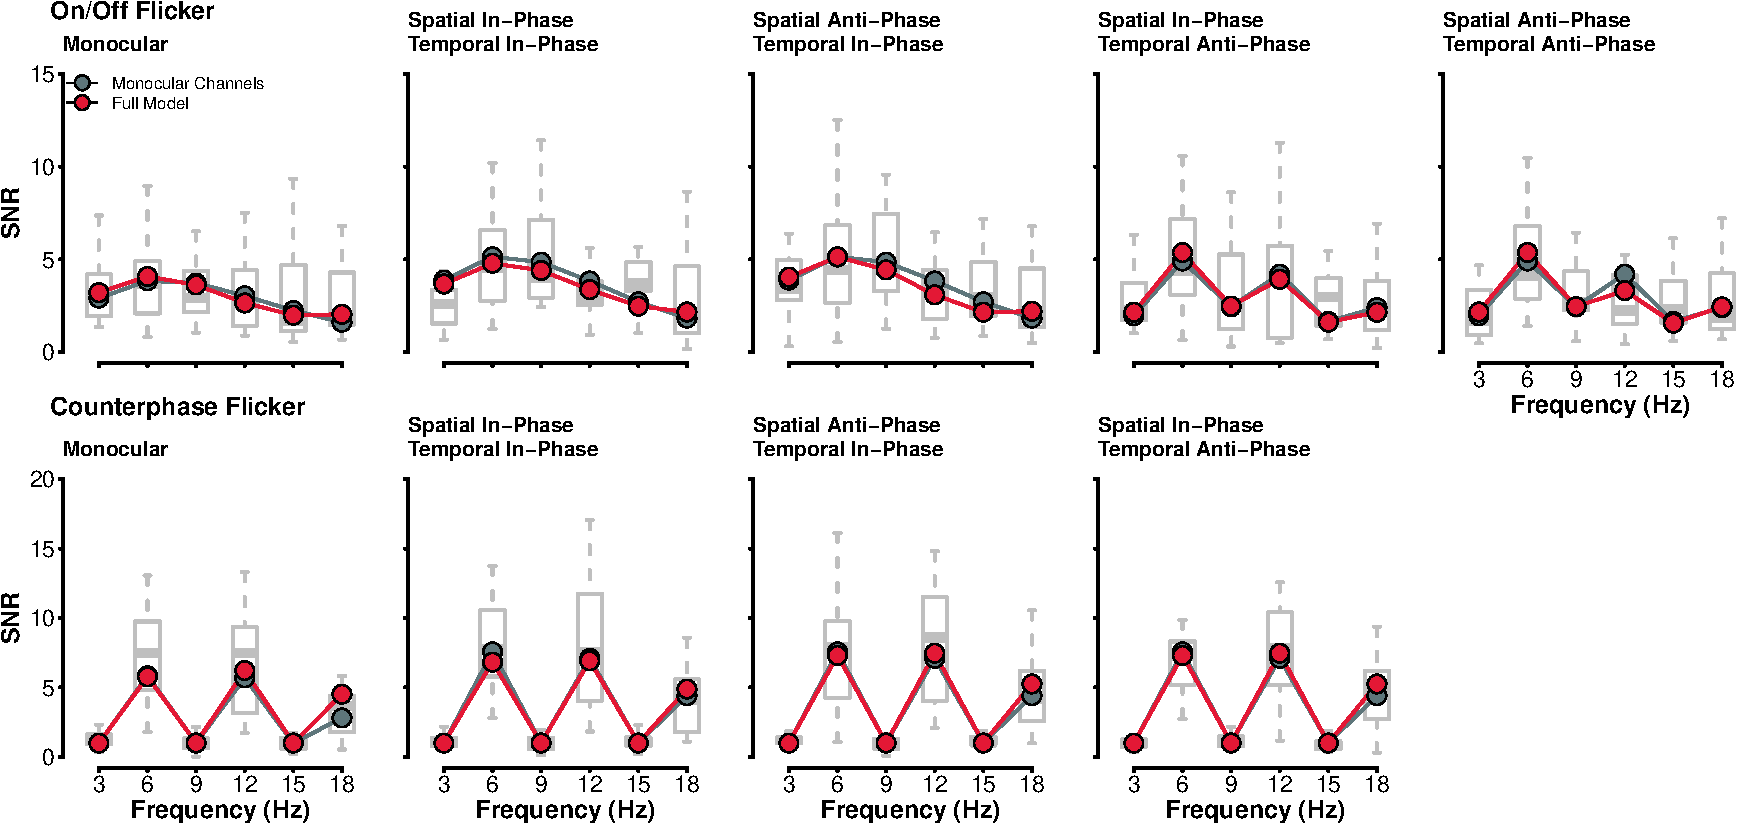
\includegraphics[keepaspectratio]{SSVEP_Phase_AntiPhase_paper_files/figure-pdf/fig-bestModels-1.pdf}}

}

\caption{\label{fig-bestModels}Fits of the two best performing models to
our observer data. Both models, that including parallel monocular
channels and the full model with the added phase-selective channels
perform quite similarly.}

\end{figure}%

Our results do not show a strong effect of stimulus spatial phase on
observer SSVEPs, nevertheless, we thought it prudent to verify if the
addition of phase-selective channels could further improve fits to our
data. We added phase-selectivity to the binocular and monocular channels
in the two-stage contrast gain control model, which required replicating
the equations from both stages to have binocular and monocular channels
selective for either positive or negative phase (see
Figure~\ref{fig-modelDiagram}). The input sine waves (in temporal phase
or anti-phase) are then fed into the positive or negative phase
channels, which simulates the spatial phase of the gratings presented to
observers. Just as the parallel monocular channels, the phase-selective
channels in this model are completely independent. This model iteration,
which we refer to as the full model, is a replication of the two-stage
contrast gain control model developed by Georgeson et al. (2016).

As with the addition of monocular channels, the addition of
phase-selectivity means that we now have six final signals to contend
with: a binocular and two monocular channels selective for positive
spatial phase and a binocular and two monocular channels selective for
negative spatial phase. The Fourier amplitude of the positive and
negative phase-selective channels were summed prior to the linear
combination of the binocular and monocular channels. The final response
of the model (\(R_\text{model}\)) is therefore

The inclusion of phase-selective channels in the model did not improve
model fits. The \(R^2\) value calculated across the 6 frequencies and 9
experimental conditions was no different, if not a little lower, than
that of the model with parallel monocular channels (see
Table~\ref{tbl-R2Table}). While spatial phase significantly impacts
psychophysical measurements of binocular summation (Bacon, 1976; Baker
and Meese, 2007; Simmons, 2005), the evidence that it affects SSVEPs of
binocular combination is lacking. The largest aspect of our data to
explain was the monocular signal to temporal anti-phase stimuli, which
can explained very well without phase-selective channels.

\section{Discussion}\label{discussion}

The computational architecture of binocular combination, under the
two-stage contrast gain control model framework, has been carefully
evaluated on psychophysical data (Baker and Meese, 2007; Georgeson et
al., 2016; Meese et al., 2006), yet its ability to explain neural data
has only been explored on a limited set of stimulus conditions (Lygo et
al., 2021; Richard et al., 2018). In this study, we investigated the
effects of stimulus spatial and temporal phase on observer SSVEPs and
explored the ability of the two-stage contrast gain control model - and
its variants - to capture these effects. We found that presenting
stimuli in temporal anti-phase reduced the magnitude of responses at the
fundamental frequency (3Hz) in comparison to its temporal phase
counterpart but was not abolished. This finding indicates that, even
under binocular viewing, purely monocular signals can be measured at the
scalp with SSVEPs. Additionally, we found the two-stage contrast gain
control model with parallel monocular and phase-selective channels to
best explain observer SSVEPs across the nine experimental conditions of
this study. The addition of monocular channels was crucial to preserve
monocular signals at later stages of the model and fit the monocular
responses of the temporal anti-phase conditions. The effect of spatial
phase on SSVEPs, however, was not found to be meaningful in our data.
While spatial phase does impact binocular combination psychophysically
(Bacon, 1976; Baker and Meese, 2007; Simmons, 2005), we have little
evidence that it meaningfully altered SSVEPs in our observers.

\paragraph{Monocular signals}\label{monocular-signals}

Parallel monocular channels were added to account for adaptation
after-effects that suggest monocular signals may be preserved and
available for perception following binocular summation (Blake et al.,
1981; Moulden, 1980). While the possibility of monocular channels had
been considered (Legge, 1984), many assumed that only the binocularly
summed signal contributed to perception.

\paragraph{The modelling}\label{the-modelling}

we demonstrate that many mechanisms of binocular combination, such as
monocular non-linearities, interocular interactions, and parallel
monocular channels, are required to explain neural responses to our set
of experimental conditions.

\subsubsection{Channels}\label{channels}

\paragraph{Summing}\label{summing}

\paragraph{Monocular channels}\label{monocular-channels}

\paragraph{Difference channels}\label{difference-channels}

Difference channels would be evident in the spatial phase conditions,
but since their responses are weaker than summing channels, could it be
that they are just not large enough to be recorded by SSVEPs? Also, what
are the temporal characteristics of differencing channels? If stimuli
are presented at a 3Hz flicker, is that oscillation too fast for the
difference channels to respond? Finally, are they selective to temporal
differences as well? One eye is on the other eye is off, will that
``activate'' difference channels?

\section{Conclusion}\label{conclusion}

The two-stage contrast gain control model remains a powerful and
flexible descriptor of the architecture of binocular combination for
data collected across many experimental conditions and modalities.

\section*{References}\label{references}
\addcontentsline{toc}{section}{References}

\phantomsection\label{refs}
\begin{CSLReferences}{1}{0}
\bibitem[\citeproctext]{ref-Bacon1976}
Bacon, J.H., 1976. The interaction of dichoptically presented spatial
gratings. Vision Res 16, 337--44.
\url{https://doi.org/10.1016/0042-6989(76)90193-0}

\bibitem[\citeproctext]{ref-Baker2018}
Baker, D.H., Lygo, F.A., Meese, T.S., Georgeson, M.A., 2018. Binocular
summation revisited: Beyond \(\sqrt{2}\). Psychol Bull 144, 1186--1199.
\url{https://doi.org/10.1037/bul0000163}

\bibitem[\citeproctext]{ref-BakerMeese2007}
Baker, D.H., Meese, T.S., 2007. Binocular contrast interactions:
Dichoptic masking is not a single process. Vision Res 47, 3096--107.
\url{https://doi.org/10.1016/j.visres.2007.08.013}

\bibitem[\citeproctext]{ref-BakerMeeseGeorgeson2007}
Baker, D.H., Meese, T.S., Georgeson, M.A., 2007a. Binocular interaction:
Contrast matching and contrast discrimination are predicted by the same
model. Spat Vis 20, 397--413.
\url{https://doi.org/10.1163/156856807781503622}

\bibitem[\citeproctext]{ref-BakerMeeseHess2008}
Baker, D.H., Meese, T.S., Hess, R.F., 2008. Contrast masking in
strabismic amblyopia: Attenuation, noise, interocular suppression and
binocular summation. Vision Res 48, 1625--40.
\url{https://doi.org/10.1016/j.visres.2008.04.017}

\bibitem[\citeproctext]{ref-BakerMeeseSummers2007}
Baker, D.H., Meese, T.S., Summers, R.J., 2007b. Psychophysical evidence
for two routes to suppression before binocular summation of signals in
human vision. Neuroscience 146, 435--448.
\url{https://doi.org/10.1016/j.neuroscience.2007.01.030}

\bibitem[\citeproctext]{ref-BakerWade2017}
Baker, D.H., Wade, A.R., 2017. Evidence for an optimal algorithm
underlying signal combination in human visual cortex. Cereb Cortex 27,
254--264. \url{https://doi.org/10.1093/cercor/bhw395}

\bibitem[\citeproctext]{ref-Blake1989}
Blake, R., 1989. A neural theory of binocular rivalry. Psychol Rev 96,
145--67. \url{https://doi.org/10.1037/0033-295x.96.1.145}

\bibitem[\citeproctext]{ref-BlakeOvertonLemaStern1981}
Blake, R., Overton, R., Lema-Stern, S., 1981. Interocular transfer of
visual aftereffects. J Exp Psychol Hum Percept Perform 7, 367--81.
\url{https://doi.org/10.1037//0096-1523.7.2.367}

\bibitem[\citeproctext]{ref-BlakeWilson2011}
Blake, R., Wilson, H., 2011. Binocular vision. Vision Research 51,
754--770. \url{https://doi.org/10.1016/j.visres.2010.10.009}

\bibitem[\citeproctext]{ref-CampbellGreen1965}
Campbell, F.W., Green, D.G., 1965. Monocular versus binocular visual
acuity. Nature 208, 191--2. \url{https://doi.org/10.1038/208191a0}

\bibitem[\citeproctext]{ref-Chatrian1985}
Chatrian, G.E., Lettich, E., Nelson, P.L., 1985. Ten percent electrode
system for topographic studies of spontaneous and evoked EEG activities.
American Journal of EEG Technology 25, 83--92.
\url{https://doi.org/10.1080/00029238.1985.11080163}

\bibitem[\citeproctext]{ref-Delorme2004}
Delorme, A., Makeig, S., 2004. EEGLAB: An open source toolbox for
analysis of single-trial EEG dynamics including independent component
analysis. Journal of Neuroscience Methods 134, 9--21.
\url{https://doi.org/10.1016/J.JNEUMETH.2003.10.009}

\bibitem[\citeproctext]{ref-DingKleinLevi2013}
Ding, J., Klein, S.A., Levi, D.M., 2013. Binocular combination of phase
and contrast explained by a gain-control and gain-enhancement model. J
Vis 13, 13. \url{https://doi.org/10.1167/13.2.13}

\bibitem[\citeproctext]{ref-DingSperling2006}
Ding, J., Sperling, G., 2006. A gain-control theory of binocular
combination. Proc Natl Acad Sci U S A 103, 1141--6.
\url{https://doi.org/10.1073/pnas.0509629103}

\bibitem[\citeproctext]{ref-Georgeson2016}
Georgeson, M.A., Wallis, S.A., Meese, T.S., Baker, D.H., 2016. Contrast
and lustre: A model that accounts for eleven different forms of contrast
discrimination in binocular vision. Vision Research 129, 98--118.
\url{https://doi.org/10.1016/j.visres.2016.08.001}

\bibitem[\citeproctext]{ref-HansenHess2006}
Hansen, B.C., Hess, R.F., 2006. Discrimination of amplitude spectrum
slope in the fovea and parafovea and the local amplitude distributions
of natural scene imagery. J Vis 6, 696--711.
\url{https://doi.org/10.1167/6.7.3}

\bibitem[\citeproctext]{ref-Heeger1992}
Heeger, D.J., 1992. Normalization of cell responses in cat striate
cortex. Vis Neurosci 9, 181--97.
\url{https://doi.org/10.1017/s0952523800009640}

\bibitem[\citeproctext]{ref-Legge1984a}
Legge, G.E., 1984. Binocular contrast summation--i. Detection and
discrimination. Vision Res 24, 373--83.
\url{https://doi.org/10.1016/0042-6989(84)90063-4}

\bibitem[\citeproctext]{ref-Lygoetal2020}
Lygo, F.A., Richard, B., Wade, A.R., Morland, A.B., Baker, D.H., 2021.
Neural markers of suppression in impaired binocular vision. Neuroimage
230, 117780. \url{https://doi.org/10.1016/j.neuroimage.2021.117780}

\bibitem[\citeproctext]{ref-MaeharaGoryo2005}
Maehara, G., Goryo, K., 2005. Binocular, monocular and dichoptic pattern
masking. Optical Review 12, 76--82.
\href{https://doi.org/DOI\%2010.1007/s10043-004-0076-5}{https://doi.org/DOI
10.1007/s10043-004-0076-5}

\bibitem[\citeproctext]{ref-MeeseBaker2011}
Meese, T.S., Baker, D.H., 2011. Contrast summation across eyes and space
is revealed along the entire dipper function by a {``swiss cheese''}
stimulus. J Vis 11, 1--23. \url{https://doi.org/10.1167/11.1.23}

\bibitem[\citeproctext]{ref-Meese2006}
Meese, T.S., Georgeson, M.A., Baker, D.H., 2006. Binocular contrast
vision at and above threshold. Journal of vision 6, 1224--1243.
\url{https://doi.org/10.1167/6.11.7}

\bibitem[\citeproctext]{ref-MoradiHeeger2009}
Moradi, F., Heeger, D.J., 2009. Inter-ocular contrast normalization in
human visual cortex. J Vis 9, 13 1--22.
\url{https://doi.org/10.1167/9.3.13}

\bibitem[\citeproctext]{ref-Moulden1980}
Moulden, B., 1980. After-effects and the integration of patterns of
neural activity within a channel. Philos Trans R Soc Lond B Biol Sci
290, 39--55. \url{https://doi.org/10.1098/rstb.1980.0081}

\bibitem[\citeproctext]{ref-regan1988}
Regan, M., Regan, D., 1988. A frequency domain technique for
characterizing nonlinearities in biological systems. Journal of
theoretical biology 133, 293--317.

\bibitem[\citeproctext]{ref-Richardetal2018}
Richard, B., Chadnova, E., Baker, D.H., 2018. Binocular vision
adaptively suppresses delayed monocular signals. Neuroimage 172,
753--765. \url{https://doi.org/10.1016/j.neuroimage.2018.02.021}

\bibitem[\citeproctext]{ref-Simmons2005}
Simmons, D.R., 2005. The binocular combination of chromatic contrast.
Perception 34, 1035--1042. \url{https://doi.org/10.1068/p5279}

\bibitem[\citeproctext]{ref-SimmonsKingdom1998}
Simmons, D.R., Kingdom, F.A.A., 1998. On the binocular summation of
chromatic contrast. Vision Research 38, 1063--1071.
\url{https://doi.org/10.1016/S0042-6989(97)00272-1}

\bibitem[\citeproctext]{ref-TadmorTolhurst1994}
Tadmor, Y., Tolhurst, D.J., 1994. Discrimination of changes in the
second-order statistics of natural and synthetic images. Vision Research
34, 541--554. \url{https://doi.org/10.1016/0042-6989(94)90167-8}

\bibitem[\citeproctext]{ref-WadeBaker2025}
Wade, A.R., Baker, D.H., 2025. Measuring contrast processing in the
visual system using the steady state visually evoked potential (SSVEP).
Vision Research 231, 108614.
\url{https://doi.org/10.1016/j.visres.2025.108614}

\bibitem[\citeproctext]{ref-Wilson2003}
Wilson, H.R., 2003. Computational evidence for a rivalry hierarchy in
vision. Proceedings of the National Academy of Sciences of the United
States of America 100, 14499--14503.
\url{https://doi.org/10.1073/pnas.2333622100}

\end{CSLReferences}




\end{document}
